\documentclass[twoside]{book}

% Packages required by doxygen
\usepackage{fixltx2e}
\usepackage{calc}
\usepackage{doxygen}
\usepackage[export]{adjustbox} % also loads graphicx
\usepackage{graphicx}
\usepackage[utf8]{inputenc}
\usepackage{makeidx}
\usepackage{multicol}
\usepackage{multirow}
\PassOptionsToPackage{warn}{textcomp}
\usepackage{textcomp}
\usepackage[nointegrals]{wasysym}
\usepackage[table]{xcolor}

% Font selection
\usepackage[T1]{fontenc}
\usepackage[scaled=.90]{helvet}
\usepackage{courier}
\usepackage{amssymb}
\usepackage{sectsty}
\renewcommand{\familydefault}{\sfdefault}
\allsectionsfont{%
  \fontseries{bc}\selectfont%
  \color{darkgray}%
}
\renewcommand{\DoxyLabelFont}{%
  \fontseries{bc}\selectfont%
  \color{darkgray}%
}
\newcommand{\+}{\discretionary{\mbox{\scriptsize$\hookleftarrow$}}{}{}}

% Page & text layout
\usepackage{geometry}
\geometry{%
  a4paper,%
  top=2.5cm,%
  bottom=2.5cm,%
  left=2.5cm,%
  right=2.5cm%
}
\tolerance=750
\hfuzz=15pt
\hbadness=750
\setlength{\emergencystretch}{15pt}
\setlength{\parindent}{0cm}
\setlength{\parskip}{3ex plus 2ex minus 2ex}
\makeatletter
\renewcommand{\paragraph}{%
  \@startsection{paragraph}{4}{0ex}{-1.0ex}{1.0ex}{%
    \normalfont\normalsize\bfseries\SS@parafont%
  }%
}
\renewcommand{\subparagraph}{%
  \@startsection{subparagraph}{5}{0ex}{-1.0ex}{1.0ex}{%
    \normalfont\normalsize\bfseries\SS@subparafont%
  }%
}
\makeatother

% Headers & footers
\usepackage{fancyhdr}
\pagestyle{fancyplain}
\fancyhead[LE]{\fancyplain{}{\bfseries\thepage}}
\fancyhead[CE]{\fancyplain{}{}}
\fancyhead[RE]{\fancyplain{}{\bfseries\leftmark}}
\fancyhead[LO]{\fancyplain{}{\bfseries\rightmark}}
\fancyhead[CO]{\fancyplain{}{}}
\fancyhead[RO]{\fancyplain{}{\bfseries\thepage}}
\fancyfoot[LE]{\fancyplain{}{}}
\fancyfoot[CE]{\fancyplain{}{}}
\fancyfoot[RE]{\fancyplain{}{\bfseries\scriptsize Generated by Doxygen }}
\fancyfoot[LO]{\fancyplain{}{\bfseries\scriptsize Generated by Doxygen }}
\fancyfoot[CO]{\fancyplain{}{}}
\fancyfoot[RO]{\fancyplain{}{}}
\renewcommand{\footrulewidth}{0.4pt}
\renewcommand{\chaptermark}[1]{%
  \markboth{#1}{}%
}
\renewcommand{\sectionmark}[1]{%
  \markright{\thesection\ #1}%
}

% Indices & bibliography
\usepackage{natbib}
\usepackage[titles]{tocloft}
\setcounter{tocdepth}{3}
\setcounter{secnumdepth}{5}
\makeindex

% Hyperlinks (required, but should be loaded last)
\usepackage{ifpdf}
\ifpdf
  \usepackage[pdftex,pagebackref=true]{hyperref}
\else
  \usepackage[ps2pdf,pagebackref=true]{hyperref}
\fi
\hypersetup{%
  colorlinks=true,%
  linkcolor=blue,%
  citecolor=blue,%
  unicode%
}

% Custom commands
\newcommand{\clearemptydoublepage}{%
  \newpage{\pagestyle{empty}\cleardoublepage}%
}

\usepackage{caption}
\captionsetup{labelsep=space,justification=centering,font={bf},singlelinecheck=off,skip=4pt,position=top}

%===== C O N T E N T S =====

\begin{document}

% Titlepage & ToC
\hypersetup{pageanchor=false,
             bookmarksnumbered=true,
             pdfencoding=unicode
            }
\pagenumbering{alph}
\begin{titlepage}
\vspace*{7cm}
\begin{center}%
{\Large W\+RC -\/ Home Challenge -\/ Merrimac }\\
\vspace*{1cm}
{\large Generated by Doxygen 1.8.14}\\
\end{center}
\end{titlepage}
\clearemptydoublepage
\pagenumbering{roman}
\tableofcontents
\clearemptydoublepage
\pagenumbering{arabic}
\hypersetup{pageanchor=true}

%--- Begin generated contents ---
\chapter{Namespace Index}
\section{Namespace List}
Here is a list of all namespaces with brief descriptions\+:\begin{DoxyCompactList}
\item\contentsline{section}{\mbox{\hyperlink{namespace_arm}{Arm}} }{\pageref{namespace_arm}}{}
\item\contentsline{section}{\mbox{\hyperlink{namespacecheck__pins}{check\+\_\+pins}} }{\pageref{namespacecheck__pins}}{}
\item\contentsline{section}{\mbox{\hyperlink{namespaceclean__up}{clean\+\_\+up}} }{\pageref{namespaceclean__up}}{}
\item\contentsline{section}{\mbox{\hyperlink{namespacecontroller}{controller}} }{\pageref{namespacecontroller}}{}
\item\contentsline{section}{\mbox{\hyperlink{namespace_motor}{Motor}} }{\pageref{namespace_motor}}{}
\item\contentsline{section}{\mbox{\hyperlink{namespace_robot}{Robot}} }{\pageref{namespace_robot}}{}
\item\contentsline{section}{\mbox{\hyperlink{namespace_ultrasonic__sensors}{Ultrasonic\+\_\+sensors}} }{\pageref{namespace_ultrasonic__sensors}}{}
\item\contentsline{section}{\mbox{\hyperlink{namespace_wheels}{Wheels}} }{\pageref{namespace_wheels}}{}
\end{DoxyCompactList}

\chapter{Hierarchical Index}
\section{Class Hierarchy}
This inheritance list is sorted roughly, but not completely, alphabetically\+:\begin{DoxyCompactList}
\item \contentsline{section}{Arm.\+Arm}{\pageref{class_arm_1_1_arm}}{}
\item \contentsline{section}{Motor.\+Motor}{\pageref{class_motor_1_1_motor}}{}
\item \contentsline{section}{Robot.\+Robot}{\pageref{class_robot_1_1_robot}}{}
\item Thread\begin{DoxyCompactList}
\item \contentsline{section}{controller.\+Control\+\_\+\+Thread}{\pageref{classcontroller_1_1_control___thread}}{}
\item \contentsline{section}{Motor.\+Motor\+\_\+\+Thread}{\pageref{class_motor_1_1_motor___thread}}{}
\item \contentsline{section}{Ultrasonic\+\_\+sensors.\+Main\+\_\+\+Thread}{\pageref{class_ultrasonic__sensors_1_1_main___thread}}{}
\item \contentsline{section}{Ultrasonic\+\_\+sensors.\+Ultrasonic\+\_\+\+Sensor\+\_\+\+Thread}{\pageref{class_ultrasonic__sensors_1_1_ultrasonic___sensor___thread}}{}
\end{DoxyCompactList}
\item \contentsline{section}{Ultrasonic\+\_\+sensors.\+Ultrasonic\+\_\+\+Sensor}{\pageref{class_ultrasonic__sensors_1_1_ultrasonic___sensor}}{}
\item \contentsline{section}{Wheels.\+Wheels}{\pageref{class_wheels_1_1_wheels}}{}
\end{DoxyCompactList}

\chapter{Class Index}
\section{Class List}
Here are the classes, structs, unions and interfaces with brief descriptions\+:\begin{DoxyCompactList}
\item\contentsline{section}{\mbox{\hyperlink{class_arm_1_1_arm}{Arm.\+Arm}} }{\pageref{class_arm_1_1_arm}}{}
\item\contentsline{section}{\mbox{\hyperlink{classcontroller_1_1_control___thread}{controller.\+Control\+\_\+\+Thread}} }{\pageref{classcontroller_1_1_control___thread}}{}
\item\contentsline{section}{\mbox{\hyperlink{class_ultrasonic__sensors_1_1_main___thread}{Ultrasonic\+\_\+sensors.\+Main\+\_\+\+Thread}} }{\pageref{class_ultrasonic__sensors_1_1_main___thread}}{}
\item\contentsline{section}{\mbox{\hyperlink{class_motor_1_1_motor}{Motor.\+Motor}} }{\pageref{class_motor_1_1_motor}}{}
\item\contentsline{section}{\mbox{\hyperlink{class_motor_1_1_motor___thread}{Motor.\+Motor\+\_\+\+Thread}} }{\pageref{class_motor_1_1_motor___thread}}{}
\item\contentsline{section}{\mbox{\hyperlink{class_robot_1_1_robot}{Robot.\+Robot}} }{\pageref{class_robot_1_1_robot}}{}
\item\contentsline{section}{\mbox{\hyperlink{class_ultrasonic__sensors_1_1_ultrasonic___sensor}{Ultrasonic\+\_\+sensors.\+Ultrasonic\+\_\+\+Sensor}} }{\pageref{class_ultrasonic__sensors_1_1_ultrasonic___sensor}}{}
\item\contentsline{section}{\mbox{\hyperlink{class_ultrasonic__sensors_1_1_ultrasonic___sensor___thread}{Ultrasonic\+\_\+sensors.\+Ultrasonic\+\_\+\+Sensor\+\_\+\+Thread}} }{\pageref{class_ultrasonic__sensors_1_1_ultrasonic___sensor___thread}}{}
\item\contentsline{section}{\mbox{\hyperlink{class_wheels_1_1_wheels}{Wheels.\+Wheels}} }{\pageref{class_wheels_1_1_wheels}}{}
\end{DoxyCompactList}

\chapter{File Index}
\section{File List}
Here is a list of all files with brief descriptions\+:\begin{DoxyCompactList}
\item\contentsline{section}{\mbox{\hyperlink{_arm_8py}{Arm.\+py}} }{\pageref{_arm_8py}}{}
\item\contentsline{section}{\mbox{\hyperlink{check__pins_8py}{check\+\_\+pins.\+py}} }{\pageref{check__pins_8py}}{}
\item\contentsline{section}{\mbox{\hyperlink{clean__up_8py}{clean\+\_\+up.\+py}} }{\pageref{clean__up_8py}}{}
\item\contentsline{section}{\mbox{\hyperlink{controller_8py}{controller.\+py}} }{\pageref{controller_8py}}{}
\item\contentsline{section}{\mbox{\hyperlink{_motor_8py}{Motor.\+py}} }{\pageref{_motor_8py}}{}
\item\contentsline{section}{\mbox{\hyperlink{_robot_8py}{Robot.\+py}} }{\pageref{_robot_8py}}{}
\item\contentsline{section}{\mbox{\hyperlink{_ultrasonic__sensors_8py}{Ultrasonic\+\_\+sensors.\+py}} }{\pageref{_ultrasonic__sensors_8py}}{}
\item\contentsline{section}{\mbox{\hyperlink{_wheels_8py}{Wheels.\+py}} }{\pageref{_wheels_8py}}{}
\end{DoxyCompactList}

\chapter{Namespace Documentation}
\hypertarget{namespace_arm}{}\section{Arm Namespace Reference}
\label{namespace_arm}\index{Arm@{Arm}}
\subsection*{Classes}
\begin{DoxyCompactItemize}
\item 
class \mbox{\hyperlink{class_arm_1_1_arm}{Arm}}
\end{DoxyCompactItemize}

\hypertarget{namespacecheck__pins}{}\section{check\+\_\+pins Namespace Reference}
\label{namespacecheck__pins}\index{check\+\_\+pins@{check\+\_\+pins}}
\subsection*{Variables}
\begin{DoxyCompactItemize}
\item 
list \mbox{\hyperlink{namespacecheck__pins_ae7e56ca97a6e158edc4836330a89f5bb}{pins}} = \mbox{[}31, 33, 35, 37, 24, 26\mbox{]}
\end{DoxyCompactItemize}


\subsection{Variable Documentation}
\mbox{\Hypertarget{namespacecheck__pins_ae7e56ca97a6e158edc4836330a89f5bb}\label{namespacecheck__pins_ae7e56ca97a6e158edc4836330a89f5bb}} 
\index{check\+\_\+pins@{check\+\_\+pins}!pins@{pins}}
\index{pins@{pins}!check\+\_\+pins@{check\+\_\+pins}}
\subsubsection{\texorpdfstring{pins}{pins}}
{\footnotesize\ttfamily list check\+\_\+pins.\+pins = \mbox{[}31, 33, 35, 37, 24, 26\mbox{]}}


\hypertarget{namespaceclean__up}{}\section{clean\+\_\+up Namespace Reference}
\label{namespaceclean__up}\index{clean\+\_\+up@{clean\+\_\+up}}

\hypertarget{namespacecontroller}{}\section{controller Namespace Reference}
\label{namespacecontroller}\index{controller@{controller}}
\subsection*{Classes}
\begin{DoxyCompactItemize}
\item 
class \mbox{\hyperlink{classcontroller_1_1_control___thread}{Control\+\_\+\+Thread}}
\end{DoxyCompactItemize}
\subsection*{Variables}
\begin{DoxyCompactItemize}
\item 
\mbox{\hyperlink{namespacecontroller_accafb331d0342effadbbe3609c156598}{left\+\_\+motor}} = \mbox{\hyperlink{class_motor_1_1_motor}{Motor.\+Motor}}(31, 33, 24)
\item 
\mbox{\hyperlink{namespacecontroller_a6d0f4d0ae0b1cc7e69b7094cec5d44e9}{left\+\_\+motor\+\_\+t}} = \mbox{\hyperlink{class_motor_1_1_motor___thread}{Motor.\+Motor\+\_\+\+Thread}}(\mbox{\hyperlink{namespacecontroller_accafb331d0342effadbbe3609c156598}{left\+\_\+motor}})
\item 
\mbox{\hyperlink{namespacecontroller_a01c7aa0aed71e493785716166c882f4f}{right\+\_\+motor}} = \mbox{\hyperlink{class_motor_1_1_motor}{Motor.\+Motor}}(35, 37, 26)
\item 
\mbox{\hyperlink{namespacecontroller_a6256e3281526776faed48e0dbfb596ec}{right\+\_\+motor\+\_\+t}} = \mbox{\hyperlink{class_motor_1_1_motor___thread}{Motor.\+Motor\+\_\+\+Thread}}(\mbox{\hyperlink{namespacecontroller_a01c7aa0aed71e493785716166c882f4f}{right\+\_\+motor}})
\item 
\mbox{\hyperlink{namespacecontroller_ac1696e3b9bdd35da786bc99515eee2b9}{wheels}} = \mbox{\hyperlink{class_wheels_1_1_wheels}{Wheels.\+Wheels}}(\mbox{\hyperlink{namespacecontroller_accafb331d0342effadbbe3609c156598}{left\+\_\+motor}}, \mbox{\hyperlink{namespacecontroller_a01c7aa0aed71e493785716166c882f4f}{right\+\_\+motor}})
\item 
\mbox{\hyperlink{namespacecontroller_a189bd3b1eaf031673385cc627be55bee}{sensor\+\_\+values}} = dict()
\item 
int \mbox{\hyperlink{namespacecontroller_a0875b114513cfcd900f5969aa48e9e91}{rate}} = 1
\item 
\mbox{\hyperlink{namespacecontroller_a16bd60420374c0595e623e0f1706972a}{robot}} = \mbox{\hyperlink{class_robot_1_1_robot}{Robot.\+Robot}}(\mbox{\hyperlink{namespacecontroller_ac1696e3b9bdd35da786bc99515eee2b9}{wheels}}, \mbox{\hyperlink{namespacecontroller_a189bd3b1eaf031673385cc627be55bee}{sensor\+\_\+values}})
\item 
\mbox{\hyperlink{namespacecontroller_a2445f7bc86ae8711053f9fe3bd4db5a9}{c\+\_\+t}} = \mbox{\hyperlink{classcontroller_1_1_control___thread}{Control\+\_\+\+Thread}}(\mbox{\hyperlink{namespacecontroller_a16bd60420374c0595e623e0f1706972a}{robot}})
\end{DoxyCompactItemize}


\subsection{Variable Documentation}
\mbox{\Hypertarget{namespacecontroller_a2445f7bc86ae8711053f9fe3bd4db5a9}\label{namespacecontroller_a2445f7bc86ae8711053f9fe3bd4db5a9}} 
\index{controller@{controller}!c\+\_\+t@{c\+\_\+t}}
\index{c\+\_\+t@{c\+\_\+t}!controller@{controller}}
\subsubsection{\texorpdfstring{c\+\_\+t}{c\_t}}
{\footnotesize\ttfamily controller.\+c\+\_\+t = \mbox{\hyperlink{classcontroller_1_1_control___thread}{Control\+\_\+\+Thread}}(\mbox{\hyperlink{namespacecontroller_a16bd60420374c0595e623e0f1706972a}{robot}})}

\mbox{\Hypertarget{namespacecontroller_accafb331d0342effadbbe3609c156598}\label{namespacecontroller_accafb331d0342effadbbe3609c156598}} 
\index{controller@{controller}!left\+\_\+motor@{left\+\_\+motor}}
\index{left\+\_\+motor@{left\+\_\+motor}!controller@{controller}}
\subsubsection{\texorpdfstring{left\+\_\+motor}{left\_motor}}
{\footnotesize\ttfamily controller.\+left\+\_\+motor = \mbox{\hyperlink{class_motor_1_1_motor}{Motor.\+Motor}}(31, 33, 24)}

\mbox{\Hypertarget{namespacecontroller_a6d0f4d0ae0b1cc7e69b7094cec5d44e9}\label{namespacecontroller_a6d0f4d0ae0b1cc7e69b7094cec5d44e9}} 
\index{controller@{controller}!left\+\_\+motor\+\_\+t@{left\+\_\+motor\+\_\+t}}
\index{left\+\_\+motor\+\_\+t@{left\+\_\+motor\+\_\+t}!controller@{controller}}
\subsubsection{\texorpdfstring{left\+\_\+motor\+\_\+t}{left\_motor\_t}}
{\footnotesize\ttfamily controller.\+left\+\_\+motor\+\_\+t = \mbox{\hyperlink{class_motor_1_1_motor___thread}{Motor.\+Motor\+\_\+\+Thread}}(\mbox{\hyperlink{namespacecontroller_accafb331d0342effadbbe3609c156598}{left\+\_\+motor}})}

\mbox{\Hypertarget{namespacecontroller_a0875b114513cfcd900f5969aa48e9e91}\label{namespacecontroller_a0875b114513cfcd900f5969aa48e9e91}} 
\index{controller@{controller}!rate@{rate}}
\index{rate@{rate}!controller@{controller}}
\subsubsection{\texorpdfstring{rate}{rate}}
{\footnotesize\ttfamily int controller.\+rate = 1}

\mbox{\Hypertarget{namespacecontroller_a01c7aa0aed71e493785716166c882f4f}\label{namespacecontroller_a01c7aa0aed71e493785716166c882f4f}} 
\index{controller@{controller}!right\+\_\+motor@{right\+\_\+motor}}
\index{right\+\_\+motor@{right\+\_\+motor}!controller@{controller}}
\subsubsection{\texorpdfstring{right\+\_\+motor}{right\_motor}}
{\footnotesize\ttfamily controller.\+right\+\_\+motor = \mbox{\hyperlink{class_motor_1_1_motor}{Motor.\+Motor}}(35, 37, 26)}

\mbox{\Hypertarget{namespacecontroller_a6256e3281526776faed48e0dbfb596ec}\label{namespacecontroller_a6256e3281526776faed48e0dbfb596ec}} 
\index{controller@{controller}!right\+\_\+motor\+\_\+t@{right\+\_\+motor\+\_\+t}}
\index{right\+\_\+motor\+\_\+t@{right\+\_\+motor\+\_\+t}!controller@{controller}}
\subsubsection{\texorpdfstring{right\+\_\+motor\+\_\+t}{right\_motor\_t}}
{\footnotesize\ttfamily controller.\+right\+\_\+motor\+\_\+t = \mbox{\hyperlink{class_motor_1_1_motor___thread}{Motor.\+Motor\+\_\+\+Thread}}(\mbox{\hyperlink{namespacecontroller_a01c7aa0aed71e493785716166c882f4f}{right\+\_\+motor}})}

\mbox{\Hypertarget{namespacecontroller_a16bd60420374c0595e623e0f1706972a}\label{namespacecontroller_a16bd60420374c0595e623e0f1706972a}} 
\index{controller@{controller}!robot@{robot}}
\index{robot@{robot}!controller@{controller}}
\subsubsection{\texorpdfstring{robot}{robot}}
{\footnotesize\ttfamily controller.\+robot = \mbox{\hyperlink{class_robot_1_1_robot}{Robot.\+Robot}}(\mbox{\hyperlink{namespacecontroller_ac1696e3b9bdd35da786bc99515eee2b9}{wheels}}, \mbox{\hyperlink{namespacecontroller_a189bd3b1eaf031673385cc627be55bee}{sensor\+\_\+values}})}

\mbox{\Hypertarget{namespacecontroller_a189bd3b1eaf031673385cc627be55bee}\label{namespacecontroller_a189bd3b1eaf031673385cc627be55bee}} 
\index{controller@{controller}!sensor\+\_\+values@{sensor\+\_\+values}}
\index{sensor\+\_\+values@{sensor\+\_\+values}!controller@{controller}}
\subsubsection{\texorpdfstring{sensor\+\_\+values}{sensor\_values}}
{\footnotesize\ttfamily controller.\+sensor\+\_\+values = dict()}

\mbox{\Hypertarget{namespacecontroller_ac1696e3b9bdd35da786bc99515eee2b9}\label{namespacecontroller_ac1696e3b9bdd35da786bc99515eee2b9}} 
\index{controller@{controller}!wheels@{wheels}}
\index{wheels@{wheels}!controller@{controller}}
\subsubsection{\texorpdfstring{wheels}{wheels}}
{\footnotesize\ttfamily controller.\+wheels = \mbox{\hyperlink{class_wheels_1_1_wheels}{Wheels.\+Wheels}}(\mbox{\hyperlink{namespacecontroller_accafb331d0342effadbbe3609c156598}{left\+\_\+motor}}, \mbox{\hyperlink{namespacecontroller_a01c7aa0aed71e493785716166c882f4f}{right\+\_\+motor}})}


\hypertarget{namespace_motor}{}\section{Motor Namespace Reference}
\label{namespace_motor}\index{Motor@{Motor}}
\subsection*{Classes}
\begin{DoxyCompactItemize}
\item 
class \mbox{\hyperlink{class_motor_1_1_motor}{Motor}}
\item 
class \mbox{\hyperlink{class_motor_1_1_motor___thread}{Motor\+\_\+\+Thread}}
\end{DoxyCompactItemize}

\hypertarget{namespace_robot}{}\section{Robot Namespace Reference}
\label{namespace_robot}\index{Robot@{Robot}}
\subsection*{Classes}
\begin{DoxyCompactItemize}
\item 
class \mbox{\hyperlink{class_robot_1_1_robot}{Robot}}
\end{DoxyCompactItemize}

\hypertarget{namespace_ultrasonic__sensors}{}\section{Ultrasonic\+\_\+sensors Namespace Reference}
\label{namespace_ultrasonic__sensors}\index{Ultrasonic\+\_\+sensors@{Ultrasonic\+\_\+sensors}}
\subsection*{Classes}
\begin{DoxyCompactItemize}
\item 
class \mbox{\hyperlink{class_ultrasonic__sensors_1_1_main___thread}{Main\+\_\+\+Thread}}
\item 
class \mbox{\hyperlink{class_ultrasonic__sensors_1_1_ultrasonic___sensor}{Ultrasonic\+\_\+\+Sensor}}
\item 
class \mbox{\hyperlink{class_ultrasonic__sensors_1_1_ultrasonic___sensor___thread}{Ultrasonic\+\_\+\+Sensor\+\_\+\+Thread}}
\end{DoxyCompactItemize}
\subsection*{Functions}
\begin{DoxyCompactItemize}
\item 
def \mbox{\hyperlink{namespace_ultrasonic__sensors_aaab4452438d0023b72bc848ae679881d}{get\+\_\+sensor\+\_\+info}} ()
\item 
def \mbox{\hyperlink{namespace_ultrasonic__sensors_a57e901bee678edc609c318cdb0cc0bc3}{setup}} (rate, sensor\+\_\+values)
\end{DoxyCompactItemize}


\subsection{Detailed Description}
\begin{DoxyVerb}    Author: Lochie Ashcroft

    Multithreaded ultrasonic sensors
    Reads sensor config from sensors.cfg
    Distance values are stored in a dictionary {id:value}
\end{DoxyVerb}
 

\subsection{Function Documentation}
\mbox{\Hypertarget{namespace_ultrasonic__sensors_aaab4452438d0023b72bc848ae679881d}\label{namespace_ultrasonic__sensors_aaab4452438d0023b72bc848ae679881d}} 
\index{Ultrasonic\+\_\+sensors@{Ultrasonic\+\_\+sensors}!get\+\_\+sensor\+\_\+info@{get\+\_\+sensor\+\_\+info}}
\index{get\+\_\+sensor\+\_\+info@{get\+\_\+sensor\+\_\+info}!Ultrasonic\+\_\+sensors@{Ultrasonic\+\_\+sensors}}
\subsubsection{\texorpdfstring{get\+\_\+sensor\+\_\+info()}{get\_sensor\_info()}}
{\footnotesize\ttfamily def Ultrasonic\+\_\+sensors.\+get\+\_\+sensor\+\_\+info (\begin{DoxyParamCaption}{ }\end{DoxyParamCaption})}

\mbox{\Hypertarget{namespace_ultrasonic__sensors_a57e901bee678edc609c318cdb0cc0bc3}\label{namespace_ultrasonic__sensors_a57e901bee678edc609c318cdb0cc0bc3}} 
\index{Ultrasonic\+\_\+sensors@{Ultrasonic\+\_\+sensors}!setup@{setup}}
\index{setup@{setup}!Ultrasonic\+\_\+sensors@{Ultrasonic\+\_\+sensors}}
\subsubsection{\texorpdfstring{setup()}{setup()}}
{\footnotesize\ttfamily def Ultrasonic\+\_\+sensors.\+setup (\begin{DoxyParamCaption}\item[{}]{rate,  }\item[{}]{sensor\+\_\+values }\end{DoxyParamCaption})}


\hypertarget{namespace_wheels}{}\section{Wheels Namespace Reference}
\label{namespace_wheels}\index{Wheels@{Wheels}}
\subsection*{Classes}
\begin{DoxyCompactItemize}
\item 
class \mbox{\hyperlink{class_wheels_1_1_wheels}{Wheels}}
\end{DoxyCompactItemize}

\chapter{Class Documentation}
\hypertarget{class_arm_1_1_arm}{}\section{Arm.\+Arm Class Reference}
\label{class_arm_1_1_arm}\index{Arm.\+Arm@{Arm.\+Arm}}
\subsection*{Public Member Functions}
\begin{DoxyCompactItemize}
\item 
def \mbox{\hyperlink{class_arm_1_1_arm_aa824d8a53e7d3eefe3318654d318290e}{\+\_\+\+\_\+init\+\_\+\+\_\+}} (self, \mbox{\hyperlink{class_arm_1_1_arm_a921108ed0eca55348c01811141009fdf}{a}}, \mbox{\hyperlink{class_arm_1_1_arm_a0cc68385222efa1318c95a5d1226773c}{b}}, \mbox{\hyperlink{class_arm_1_1_arm_ab07711ba5be70642e2cc07fe4e749722}{claw}})
\item 
def \mbox{\hyperlink{class_arm_1_1_arm_ad71a3d5f203842673fab1446ed5fa4d0}{extend\+\_\+arm}} (self)
\item 
def \mbox{\hyperlink{class_arm_1_1_arm_ad80e96cf9cba7fc35c0e2b3bc5c20521}{retract\+\_\+arm}} (self)
\item 
def \mbox{\hyperlink{class_arm_1_1_arm_a8044b0ae39c9d1557263e2bc7e8a6458}{extend\+\_\+a}} (self)
\item 
def \mbox{\hyperlink{class_arm_1_1_arm_a2cb928c3f4875e20c3f1a86e303349c5}{extend\+\_\+b}} (self)
\item 
def \mbox{\hyperlink{class_arm_1_1_arm_adc6b66c321eb919da68759ab0cceb1f9}{grip}} (self)
\item 
def \mbox{\hyperlink{class_arm_1_1_arm_a8f91c12bc43bd155d903bebed7ddf7ad}{un\+\_\+grip}} (self)
\item 
def \mbox{\hyperlink{class_arm_1_1_arm_ab5d57caa9e3c9ba55f03c75216e659d4}{retract\+\_\+a}} (self)
\item 
def \mbox{\hyperlink{class_arm_1_1_arm_a0bee7d96a870674ecce215bbd4faf1d5}{retract\+\_\+b}} (self)
\end{DoxyCompactItemize}
\subsection*{Public Attributes}
\begin{DoxyCompactItemize}
\item 
\mbox{\hyperlink{class_arm_1_1_arm_a921108ed0eca55348c01811141009fdf}{a}}
\item 
\mbox{\hyperlink{class_arm_1_1_arm_a0cc68385222efa1318c95a5d1226773c}{b}}
\item 
\mbox{\hyperlink{class_arm_1_1_arm_ab07711ba5be70642e2cc07fe4e749722}{claw}}
\end{DoxyCompactItemize}


\subsection{Detailed Description}
\begin{DoxyVerb}Wrapper around 3 motors, a, b, and a claw
\end{DoxyVerb}
 

\subsection{Constructor \& Destructor Documentation}
\mbox{\Hypertarget{class_arm_1_1_arm_aa824d8a53e7d3eefe3318654d318290e}\label{class_arm_1_1_arm_aa824d8a53e7d3eefe3318654d318290e}} 
\index{Arm\+::\+Arm@{Arm\+::\+Arm}!\+\_\+\+\_\+init\+\_\+\+\_\+@{\+\_\+\+\_\+init\+\_\+\+\_\+}}
\index{\+\_\+\+\_\+init\+\_\+\+\_\+@{\+\_\+\+\_\+init\+\_\+\+\_\+}!Arm\+::\+Arm@{Arm\+::\+Arm}}
\subsubsection{\texorpdfstring{\+\_\+\+\_\+init\+\_\+\+\_\+()}{\_\_init\_\_()}}
{\footnotesize\ttfamily def Arm.\+Arm.\+\_\+\+\_\+init\+\_\+\+\_\+ (\begin{DoxyParamCaption}\item[{}]{self,  }\item[{}]{a,  }\item[{}]{b,  }\item[{}]{claw }\end{DoxyParamCaption})}



\subsection{Member Function Documentation}
\mbox{\Hypertarget{class_arm_1_1_arm_a8044b0ae39c9d1557263e2bc7e8a6458}\label{class_arm_1_1_arm_a8044b0ae39c9d1557263e2bc7e8a6458}} 
\index{Arm\+::\+Arm@{Arm\+::\+Arm}!extend\+\_\+a@{extend\+\_\+a}}
\index{extend\+\_\+a@{extend\+\_\+a}!Arm\+::\+Arm@{Arm\+::\+Arm}}
\subsubsection{\texorpdfstring{extend\+\_\+a()}{extend\_a()}}
{\footnotesize\ttfamily def Arm.\+Arm.\+extend\+\_\+a (\begin{DoxyParamCaption}\item[{}]{self }\end{DoxyParamCaption})}

\mbox{\Hypertarget{class_arm_1_1_arm_ad71a3d5f203842673fab1446ed5fa4d0}\label{class_arm_1_1_arm_ad71a3d5f203842673fab1446ed5fa4d0}} 
\index{Arm\+::\+Arm@{Arm\+::\+Arm}!extend\+\_\+arm@{extend\+\_\+arm}}
\index{extend\+\_\+arm@{extend\+\_\+arm}!Arm\+::\+Arm@{Arm\+::\+Arm}}
\subsubsection{\texorpdfstring{extend\+\_\+arm()}{extend\_arm()}}
{\footnotesize\ttfamily def Arm.\+Arm.\+extend\+\_\+arm (\begin{DoxyParamCaption}\item[{}]{self }\end{DoxyParamCaption})}

\mbox{\Hypertarget{class_arm_1_1_arm_a2cb928c3f4875e20c3f1a86e303349c5}\label{class_arm_1_1_arm_a2cb928c3f4875e20c3f1a86e303349c5}} 
\index{Arm\+::\+Arm@{Arm\+::\+Arm}!extend\+\_\+b@{extend\+\_\+b}}
\index{extend\+\_\+b@{extend\+\_\+b}!Arm\+::\+Arm@{Arm\+::\+Arm}}
\subsubsection{\texorpdfstring{extend\+\_\+b()}{extend\_b()}}
{\footnotesize\ttfamily def Arm.\+Arm.\+extend\+\_\+b (\begin{DoxyParamCaption}\item[{}]{self }\end{DoxyParamCaption})}

\mbox{\Hypertarget{class_arm_1_1_arm_adc6b66c321eb919da68759ab0cceb1f9}\label{class_arm_1_1_arm_adc6b66c321eb919da68759ab0cceb1f9}} 
\index{Arm\+::\+Arm@{Arm\+::\+Arm}!grip@{grip}}
\index{grip@{grip}!Arm\+::\+Arm@{Arm\+::\+Arm}}
\subsubsection{\texorpdfstring{grip()}{grip()}}
{\footnotesize\ttfamily def Arm.\+Arm.\+grip (\begin{DoxyParamCaption}\item[{}]{self }\end{DoxyParamCaption})}

\mbox{\Hypertarget{class_arm_1_1_arm_ab5d57caa9e3c9ba55f03c75216e659d4}\label{class_arm_1_1_arm_ab5d57caa9e3c9ba55f03c75216e659d4}} 
\index{Arm\+::\+Arm@{Arm\+::\+Arm}!retract\+\_\+a@{retract\+\_\+a}}
\index{retract\+\_\+a@{retract\+\_\+a}!Arm\+::\+Arm@{Arm\+::\+Arm}}
\subsubsection{\texorpdfstring{retract\+\_\+a()}{retract\_a()}}
{\footnotesize\ttfamily def Arm.\+Arm.\+retract\+\_\+a (\begin{DoxyParamCaption}\item[{}]{self }\end{DoxyParamCaption})}

\mbox{\Hypertarget{class_arm_1_1_arm_ad80e96cf9cba7fc35c0e2b3bc5c20521}\label{class_arm_1_1_arm_ad80e96cf9cba7fc35c0e2b3bc5c20521}} 
\index{Arm\+::\+Arm@{Arm\+::\+Arm}!retract\+\_\+arm@{retract\+\_\+arm}}
\index{retract\+\_\+arm@{retract\+\_\+arm}!Arm\+::\+Arm@{Arm\+::\+Arm}}
\subsubsection{\texorpdfstring{retract\+\_\+arm()}{retract\_arm()}}
{\footnotesize\ttfamily def Arm.\+Arm.\+retract\+\_\+arm (\begin{DoxyParamCaption}\item[{}]{self }\end{DoxyParamCaption})}

\mbox{\Hypertarget{class_arm_1_1_arm_a0bee7d96a870674ecce215bbd4faf1d5}\label{class_arm_1_1_arm_a0bee7d96a870674ecce215bbd4faf1d5}} 
\index{Arm\+::\+Arm@{Arm\+::\+Arm}!retract\+\_\+b@{retract\+\_\+b}}
\index{retract\+\_\+b@{retract\+\_\+b}!Arm\+::\+Arm@{Arm\+::\+Arm}}
\subsubsection{\texorpdfstring{retract\+\_\+b()}{retract\_b()}}
{\footnotesize\ttfamily def Arm.\+Arm.\+retract\+\_\+b (\begin{DoxyParamCaption}\item[{}]{self }\end{DoxyParamCaption})}

\mbox{\Hypertarget{class_arm_1_1_arm_a8f91c12bc43bd155d903bebed7ddf7ad}\label{class_arm_1_1_arm_a8f91c12bc43bd155d903bebed7ddf7ad}} 
\index{Arm\+::\+Arm@{Arm\+::\+Arm}!un\+\_\+grip@{un\+\_\+grip}}
\index{un\+\_\+grip@{un\+\_\+grip}!Arm\+::\+Arm@{Arm\+::\+Arm}}
\subsubsection{\texorpdfstring{un\+\_\+grip()}{un\_grip()}}
{\footnotesize\ttfamily def Arm.\+Arm.\+un\+\_\+grip (\begin{DoxyParamCaption}\item[{}]{self }\end{DoxyParamCaption})}



\subsection{Member Data Documentation}
\mbox{\Hypertarget{class_arm_1_1_arm_a921108ed0eca55348c01811141009fdf}\label{class_arm_1_1_arm_a921108ed0eca55348c01811141009fdf}} 
\index{Arm\+::\+Arm@{Arm\+::\+Arm}!a@{a}}
\index{a@{a}!Arm\+::\+Arm@{Arm\+::\+Arm}}
\subsubsection{\texorpdfstring{a}{a}}
{\footnotesize\ttfamily Arm.\+Arm.\+a}

\mbox{\Hypertarget{class_arm_1_1_arm_a0cc68385222efa1318c95a5d1226773c}\label{class_arm_1_1_arm_a0cc68385222efa1318c95a5d1226773c}} 
\index{Arm\+::\+Arm@{Arm\+::\+Arm}!b@{b}}
\index{b@{b}!Arm\+::\+Arm@{Arm\+::\+Arm}}
\subsubsection{\texorpdfstring{b}{b}}
{\footnotesize\ttfamily Arm.\+Arm.\+b}

\mbox{\Hypertarget{class_arm_1_1_arm_ab07711ba5be70642e2cc07fe4e749722}\label{class_arm_1_1_arm_ab07711ba5be70642e2cc07fe4e749722}} 
\index{Arm\+::\+Arm@{Arm\+::\+Arm}!claw@{claw}}
\index{claw@{claw}!Arm\+::\+Arm@{Arm\+::\+Arm}}
\subsubsection{\texorpdfstring{claw}{claw}}
{\footnotesize\ttfamily Arm.\+Arm.\+claw}



The documentation for this class was generated from the following file\+:\begin{DoxyCompactItemize}
\item 
\mbox{\hyperlink{_arm_8py}{Arm.\+py}}\end{DoxyCompactItemize}

\hypertarget{classcontroller_1_1_control___thread}{}\section{controller.\+Control\+\_\+\+Thread Class Reference}
\label{classcontroller_1_1_control___thread}\index{controller.\+Control\+\_\+\+Thread@{controller.\+Control\+\_\+\+Thread}}
Inheritance diagram for controller.\+Control\+\_\+\+Thread\+:\begin{figure}[H]
\begin{center}
\leavevmode
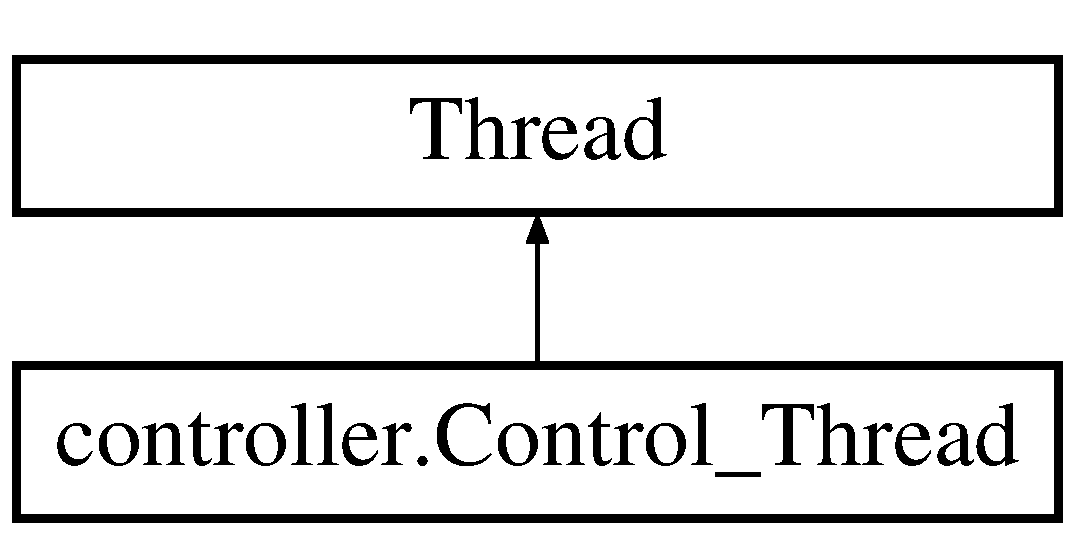
\includegraphics[height=2.000000cm]{classcontroller_1_1_control___thread}
\end{center}
\end{figure}
\subsection*{Public Member Functions}
\begin{DoxyCompactItemize}
\item 
def \mbox{\hyperlink{classcontroller_1_1_control___thread_a56f033bd2097d4fd92d5cbef29f48929}{\+\_\+\+\_\+init\+\_\+\+\_\+}} (self, \mbox{\hyperlink{classcontroller_1_1_control___thread_a4f9d431655d0036c127cc9539d5f6899}{robot}})
\item 
def \mbox{\hyperlink{classcontroller_1_1_control___thread_a56f8c6a8b6f9bf8ebc91a9a44e443993}{run}} (self)
\end{DoxyCompactItemize}
\subsection*{Public Attributes}
\begin{DoxyCompactItemize}
\item 
\mbox{\hyperlink{classcontroller_1_1_control___thread_a4f9d431655d0036c127cc9539d5f6899}{robot}}
\end{DoxyCompactItemize}


\subsection{Detailed Description}
\begin{DoxyVerb}Simple controller which takes user inputs, controls robots movements
\end{DoxyVerb}
 

\subsection{Constructor \& Destructor Documentation}
\mbox{\Hypertarget{classcontroller_1_1_control___thread_a56f033bd2097d4fd92d5cbef29f48929}\label{classcontroller_1_1_control___thread_a56f033bd2097d4fd92d5cbef29f48929}} 
\index{controller\+::\+Control\+\_\+\+Thread@{controller\+::\+Control\+\_\+\+Thread}!\+\_\+\+\_\+init\+\_\+\+\_\+@{\+\_\+\+\_\+init\+\_\+\+\_\+}}
\index{\+\_\+\+\_\+init\+\_\+\+\_\+@{\+\_\+\+\_\+init\+\_\+\+\_\+}!controller\+::\+Control\+\_\+\+Thread@{controller\+::\+Control\+\_\+\+Thread}}
\subsubsection{\texorpdfstring{\+\_\+\+\_\+init\+\_\+\+\_\+()}{\_\_init\_\_()}}
{\footnotesize\ttfamily def controller.\+Control\+\_\+\+Thread.\+\_\+\+\_\+init\+\_\+\+\_\+ (\begin{DoxyParamCaption}\item[{}]{self,  }\item[{}]{robot }\end{DoxyParamCaption})}



\subsection{Member Function Documentation}
\mbox{\Hypertarget{classcontroller_1_1_control___thread_a56f8c6a8b6f9bf8ebc91a9a44e443993}\label{classcontroller_1_1_control___thread_a56f8c6a8b6f9bf8ebc91a9a44e443993}} 
\index{controller\+::\+Control\+\_\+\+Thread@{controller\+::\+Control\+\_\+\+Thread}!run@{run}}
\index{run@{run}!controller\+::\+Control\+\_\+\+Thread@{controller\+::\+Control\+\_\+\+Thread}}
\subsubsection{\texorpdfstring{run()}{run()}}
{\footnotesize\ttfamily def controller.\+Control\+\_\+\+Thread.\+run (\begin{DoxyParamCaption}\item[{}]{self }\end{DoxyParamCaption})}



\subsection{Member Data Documentation}
\mbox{\Hypertarget{classcontroller_1_1_control___thread_a4f9d431655d0036c127cc9539d5f6899}\label{classcontroller_1_1_control___thread_a4f9d431655d0036c127cc9539d5f6899}} 
\index{controller\+::\+Control\+\_\+\+Thread@{controller\+::\+Control\+\_\+\+Thread}!robot@{robot}}
\index{robot@{robot}!controller\+::\+Control\+\_\+\+Thread@{controller\+::\+Control\+\_\+\+Thread}}
\subsubsection{\texorpdfstring{robot}{robot}}
{\footnotesize\ttfamily controller.\+Control\+\_\+\+Thread.\+robot}



The documentation for this class was generated from the following file\+:\begin{DoxyCompactItemize}
\item 
\mbox{\hyperlink{controller_8py}{controller.\+py}}\end{DoxyCompactItemize}

\hypertarget{class_ultrasonic__sensors_1_1_main___thread}{}\section{Ultrasonic\+\_\+sensors.\+Main\+\_\+\+Thread Class Reference}
\label{class_ultrasonic__sensors_1_1_main___thread}\index{Ultrasonic\+\_\+sensors.\+Main\+\_\+\+Thread@{Ultrasonic\+\_\+sensors.\+Main\+\_\+\+Thread}}
Inheritance diagram for Ultrasonic\+\_\+sensors.\+Main\+\_\+\+Thread\+:\begin{figure}[H]
\begin{center}
\leavevmode
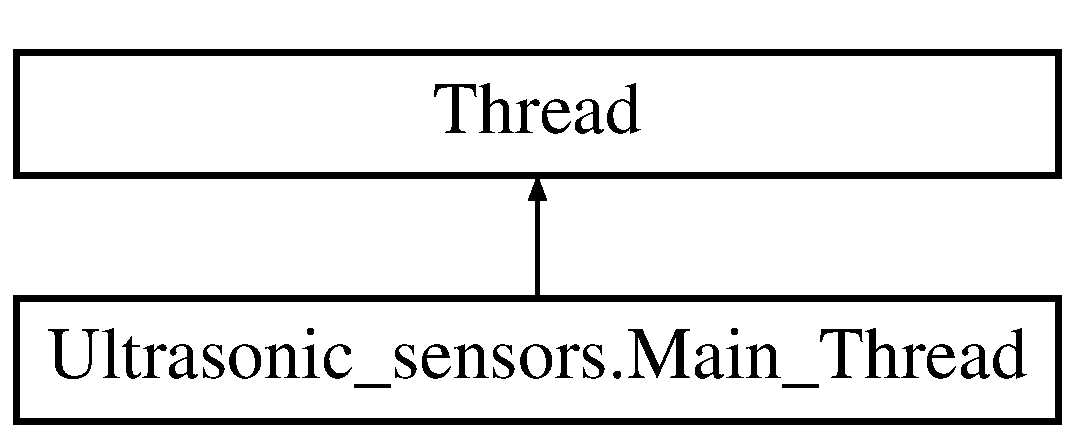
\includegraphics[height=2.000000cm]{class_ultrasonic__sensors_1_1_main___thread}
\end{center}
\end{figure}
\subsection*{Public Member Functions}
\begin{DoxyCompactItemize}
\item 
def \mbox{\hyperlink{class_ultrasonic__sensors_1_1_main___thread_ad4a11271f82f2886de7e8dac7ad06455}{\+\_\+\+\_\+init\+\_\+\+\_\+}} (self, sensor\+\_\+values)
\end{DoxyCompactItemize}


\subsection{Constructor \& Destructor Documentation}
\mbox{\Hypertarget{class_ultrasonic__sensors_1_1_main___thread_ad4a11271f82f2886de7e8dac7ad06455}\label{class_ultrasonic__sensors_1_1_main___thread_ad4a11271f82f2886de7e8dac7ad06455}} 
\index{Ultrasonic\+\_\+sensors\+::\+Main\+\_\+\+Thread@{Ultrasonic\+\_\+sensors\+::\+Main\+\_\+\+Thread}!\+\_\+\+\_\+init\+\_\+\+\_\+@{\+\_\+\+\_\+init\+\_\+\+\_\+}}
\index{\+\_\+\+\_\+init\+\_\+\+\_\+@{\+\_\+\+\_\+init\+\_\+\+\_\+}!Ultrasonic\+\_\+sensors\+::\+Main\+\_\+\+Thread@{Ultrasonic\+\_\+sensors\+::\+Main\+\_\+\+Thread}}
\subsubsection{\texorpdfstring{\+\_\+\+\_\+init\+\_\+\+\_\+()}{\_\_init\_\_()}}
{\footnotesize\ttfamily def Ultrasonic\+\_\+sensors.\+Main\+\_\+\+Thread.\+\_\+\+\_\+init\+\_\+\+\_\+ (\begin{DoxyParamCaption}\item[{}]{self,  }\item[{}]{sensor\+\_\+values }\end{DoxyParamCaption})}



The documentation for this class was generated from the following file\+:\begin{DoxyCompactItemize}
\item 
\mbox{\hyperlink{_ultrasonic__sensors_8py}{Ultrasonic\+\_\+sensors.\+py}}\end{DoxyCompactItemize}

\hypertarget{class_motor_1_1_motor}{}\section{Motor.\+Motor Class Reference}
\label{class_motor_1_1_motor}\index{Motor.\+Motor@{Motor.\+Motor}}
\subsection*{Public Member Functions}
\begin{DoxyCompactItemize}
\item 
def \mbox{\hyperlink{class_motor_1_1_motor_aaa1c1666508649052047c99cbf697e3e}{\+\_\+\+\_\+init\+\_\+\+\_\+}} (self, a, b, enable)
\item 
def \mbox{\hyperlink{class_motor_1_1_motor_a77fe4c03a7048d04172fcfca50c42e1d}{set\+\_\+speed}} (self, \mbox{\hyperlink{class_motor_1_1_motor_a73455a68e45e155c7709d1b4ec2005d6}{speed}})
\item 
def \mbox{\hyperlink{class_motor_1_1_motor_ab3b1ca0e2439d9c0f5e7c19396cac926}{get\+\_\+speed}} (self)
\item 
def \mbox{\hyperlink{class_motor_1_1_motor_a5f3b324d2803fdf965e0f4cdd5872ca6}{set\+\_\+a}} (self, state)
\item 
def \mbox{\hyperlink{class_motor_1_1_motor_a6b6473652d46b14568ba27f4b927d715}{set\+\_\+b}} (self, state)
\item 
def \mbox{\hyperlink{class_motor_1_1_motor_a24ce933b59d15a3cb77aae0dac6c8976}{get\+\_\+a}} (self)
\item 
def \mbox{\hyperlink{class_motor_1_1_motor_a606b32b1ddc5872693a482769e8e0efa}{get\+\_\+b}} (self)
\item 
def \mbox{\hyperlink{class_motor_1_1_motor_a43d6487962d166187b7c877d8dd87a40}{set\+\_\+state}} (self, state)
\item 
def \mbox{\hyperlink{class_motor_1_1_motor_a5aeb33b843755f7e96bc037afdd6794b}{get\+\_\+state}} (self)
\end{DoxyCompactItemize}
\subsection*{Public Attributes}
\begin{DoxyCompactItemize}
\item 
\mbox{\hyperlink{class_motor_1_1_motor_a9bb6737a01af43393af8adced5a478a3}{a\+\_\+pin}}
\item 
\mbox{\hyperlink{class_motor_1_1_motor_a8b625c6152a1428fd80ce08ca42440d6}{b\+\_\+pin}}
\item 
\mbox{\hyperlink{class_motor_1_1_motor_a2e4704349ae6d0a47f2d9d8e86290ffe}{enable\+\_\+pin}}
\item 
\mbox{\hyperlink{class_motor_1_1_motor_a38cf3355fa1ced6aea642b65d8f1bd5c}{a\+\_\+enabled}}
\item 
\mbox{\hyperlink{class_motor_1_1_motor_aa2e2e43d109c4711df0087a90bf3de14}{b\+\_\+enabled}}
\item 
\mbox{\hyperlink{class_motor_1_1_motor_a005d2c31df0e94b8c9002e36b8af7fba}{enabled}}
\item 
\mbox{\hyperlink{class_motor_1_1_motor_a73455a68e45e155c7709d1b4ec2005d6}{speed}}
\item 
\mbox{\hyperlink{class_motor_1_1_motor_a68d4a60b126c7b5d435dfda08d8e0c26}{pulse\+\_\+width}}
\item 
\mbox{\hyperlink{class_motor_1_1_motor_a30553a87fea4c45c7dc9a0d908d55d7c}{pulse\+\_\+high}}
\item 
\mbox{\hyperlink{class_motor_1_1_motor_a75e04d07608f99293ddafc69f5364783}{pulse\+\_\+low}}
\end{DoxyCompactItemize}


\subsection{Detailed Description}
\begin{DoxyVerb}Stores information about the motor, and sets up the pins.
Pin 'a' and 'b' are 'in1' and 'in2' on the H-Bridge, 'enable' is the 'EN' pin
\end{DoxyVerb}
 

\subsection{Constructor \& Destructor Documentation}
\mbox{\Hypertarget{class_motor_1_1_motor_aaa1c1666508649052047c99cbf697e3e}\label{class_motor_1_1_motor_aaa1c1666508649052047c99cbf697e3e}} 
\index{Motor\+::\+Motor@{Motor\+::\+Motor}!\+\_\+\+\_\+init\+\_\+\+\_\+@{\+\_\+\+\_\+init\+\_\+\+\_\+}}
\index{\+\_\+\+\_\+init\+\_\+\+\_\+@{\+\_\+\+\_\+init\+\_\+\+\_\+}!Motor\+::\+Motor@{Motor\+::\+Motor}}
\subsubsection{\texorpdfstring{\+\_\+\+\_\+init\+\_\+\+\_\+()}{\_\_init\_\_()}}
{\footnotesize\ttfamily def Motor.\+Motor.\+\_\+\+\_\+init\+\_\+\+\_\+ (\begin{DoxyParamCaption}\item[{}]{self,  }\item[{}]{a,  }\item[{}]{b,  }\item[{}]{enable }\end{DoxyParamCaption})}



\subsection{Member Function Documentation}
\mbox{\Hypertarget{class_motor_1_1_motor_a24ce933b59d15a3cb77aae0dac6c8976}\label{class_motor_1_1_motor_a24ce933b59d15a3cb77aae0dac6c8976}} 
\index{Motor\+::\+Motor@{Motor\+::\+Motor}!get\+\_\+a@{get\+\_\+a}}
\index{get\+\_\+a@{get\+\_\+a}!Motor\+::\+Motor@{Motor\+::\+Motor}}
\subsubsection{\texorpdfstring{get\+\_\+a()}{get\_a()}}
{\footnotesize\ttfamily def Motor.\+Motor.\+get\+\_\+a (\begin{DoxyParamCaption}\item[{}]{self }\end{DoxyParamCaption})}

\mbox{\Hypertarget{class_motor_1_1_motor_a606b32b1ddc5872693a482769e8e0efa}\label{class_motor_1_1_motor_a606b32b1ddc5872693a482769e8e0efa}} 
\index{Motor\+::\+Motor@{Motor\+::\+Motor}!get\+\_\+b@{get\+\_\+b}}
\index{get\+\_\+b@{get\+\_\+b}!Motor\+::\+Motor@{Motor\+::\+Motor}}
\subsubsection{\texorpdfstring{get\+\_\+b()}{get\_b()}}
{\footnotesize\ttfamily def Motor.\+Motor.\+get\+\_\+b (\begin{DoxyParamCaption}\item[{}]{self }\end{DoxyParamCaption})}

\mbox{\Hypertarget{class_motor_1_1_motor_ab3b1ca0e2439d9c0f5e7c19396cac926}\label{class_motor_1_1_motor_ab3b1ca0e2439d9c0f5e7c19396cac926}} 
\index{Motor\+::\+Motor@{Motor\+::\+Motor}!get\+\_\+speed@{get\+\_\+speed}}
\index{get\+\_\+speed@{get\+\_\+speed}!Motor\+::\+Motor@{Motor\+::\+Motor}}
\subsubsection{\texorpdfstring{get\+\_\+speed()}{get\_speed()}}
{\footnotesize\ttfamily def Motor.\+Motor.\+get\+\_\+speed (\begin{DoxyParamCaption}\item[{}]{self }\end{DoxyParamCaption})}

\mbox{\Hypertarget{class_motor_1_1_motor_a5aeb33b843755f7e96bc037afdd6794b}\label{class_motor_1_1_motor_a5aeb33b843755f7e96bc037afdd6794b}} 
\index{Motor\+::\+Motor@{Motor\+::\+Motor}!get\+\_\+state@{get\+\_\+state}}
\index{get\+\_\+state@{get\+\_\+state}!Motor\+::\+Motor@{Motor\+::\+Motor}}
\subsubsection{\texorpdfstring{get\+\_\+state()}{get\_state()}}
{\footnotesize\ttfamily def Motor.\+Motor.\+get\+\_\+state (\begin{DoxyParamCaption}\item[{}]{self }\end{DoxyParamCaption})}

\mbox{\Hypertarget{class_motor_1_1_motor_a5f3b324d2803fdf965e0f4cdd5872ca6}\label{class_motor_1_1_motor_a5f3b324d2803fdf965e0f4cdd5872ca6}} 
\index{Motor\+::\+Motor@{Motor\+::\+Motor}!set\+\_\+a@{set\+\_\+a}}
\index{set\+\_\+a@{set\+\_\+a}!Motor\+::\+Motor@{Motor\+::\+Motor}}
\subsubsection{\texorpdfstring{set\+\_\+a()}{set\_a()}}
{\footnotesize\ttfamily def Motor.\+Motor.\+set\+\_\+a (\begin{DoxyParamCaption}\item[{}]{self,  }\item[{}]{state }\end{DoxyParamCaption})}

\mbox{\Hypertarget{class_motor_1_1_motor_a6b6473652d46b14568ba27f4b927d715}\label{class_motor_1_1_motor_a6b6473652d46b14568ba27f4b927d715}} 
\index{Motor\+::\+Motor@{Motor\+::\+Motor}!set\+\_\+b@{set\+\_\+b}}
\index{set\+\_\+b@{set\+\_\+b}!Motor\+::\+Motor@{Motor\+::\+Motor}}
\subsubsection{\texorpdfstring{set\+\_\+b()}{set\_b()}}
{\footnotesize\ttfamily def Motor.\+Motor.\+set\+\_\+b (\begin{DoxyParamCaption}\item[{}]{self,  }\item[{}]{state }\end{DoxyParamCaption})}

\mbox{\Hypertarget{class_motor_1_1_motor_a77fe4c03a7048d04172fcfca50c42e1d}\label{class_motor_1_1_motor_a77fe4c03a7048d04172fcfca50c42e1d}} 
\index{Motor\+::\+Motor@{Motor\+::\+Motor}!set\+\_\+speed@{set\+\_\+speed}}
\index{set\+\_\+speed@{set\+\_\+speed}!Motor\+::\+Motor@{Motor\+::\+Motor}}
\subsubsection{\texorpdfstring{set\+\_\+speed()}{set\_speed()}}
{\footnotesize\ttfamily def Motor.\+Motor.\+set\+\_\+speed (\begin{DoxyParamCaption}\item[{}]{self,  }\item[{}]{speed }\end{DoxyParamCaption})}

\begin{DoxyVerb}Speeds of -100 to 100, negative being reverse
\end{DoxyVerb}
 \mbox{\Hypertarget{class_motor_1_1_motor_a43d6487962d166187b7c877d8dd87a40}\label{class_motor_1_1_motor_a43d6487962d166187b7c877d8dd87a40}} 
\index{Motor\+::\+Motor@{Motor\+::\+Motor}!set\+\_\+state@{set\+\_\+state}}
\index{set\+\_\+state@{set\+\_\+state}!Motor\+::\+Motor@{Motor\+::\+Motor}}
\subsubsection{\texorpdfstring{set\+\_\+state()}{set\_state()}}
{\footnotesize\ttfamily def Motor.\+Motor.\+set\+\_\+state (\begin{DoxyParamCaption}\item[{}]{self,  }\item[{}]{state }\end{DoxyParamCaption})}



\subsection{Member Data Documentation}
\mbox{\Hypertarget{class_motor_1_1_motor_a38cf3355fa1ced6aea642b65d8f1bd5c}\label{class_motor_1_1_motor_a38cf3355fa1ced6aea642b65d8f1bd5c}} 
\index{Motor\+::\+Motor@{Motor\+::\+Motor}!a\+\_\+enabled@{a\+\_\+enabled}}
\index{a\+\_\+enabled@{a\+\_\+enabled}!Motor\+::\+Motor@{Motor\+::\+Motor}}
\subsubsection{\texorpdfstring{a\+\_\+enabled}{a\_enabled}}
{\footnotesize\ttfamily Motor.\+Motor.\+a\+\_\+enabled}

\mbox{\Hypertarget{class_motor_1_1_motor_a9bb6737a01af43393af8adced5a478a3}\label{class_motor_1_1_motor_a9bb6737a01af43393af8adced5a478a3}} 
\index{Motor\+::\+Motor@{Motor\+::\+Motor}!a\+\_\+pin@{a\+\_\+pin}}
\index{a\+\_\+pin@{a\+\_\+pin}!Motor\+::\+Motor@{Motor\+::\+Motor}}
\subsubsection{\texorpdfstring{a\+\_\+pin}{a\_pin}}
{\footnotesize\ttfamily Motor.\+Motor.\+a\+\_\+pin}

\mbox{\Hypertarget{class_motor_1_1_motor_aa2e2e43d109c4711df0087a90bf3de14}\label{class_motor_1_1_motor_aa2e2e43d109c4711df0087a90bf3de14}} 
\index{Motor\+::\+Motor@{Motor\+::\+Motor}!b\+\_\+enabled@{b\+\_\+enabled}}
\index{b\+\_\+enabled@{b\+\_\+enabled}!Motor\+::\+Motor@{Motor\+::\+Motor}}
\subsubsection{\texorpdfstring{b\+\_\+enabled}{b\_enabled}}
{\footnotesize\ttfamily Motor.\+Motor.\+b\+\_\+enabled}

\mbox{\Hypertarget{class_motor_1_1_motor_a8b625c6152a1428fd80ce08ca42440d6}\label{class_motor_1_1_motor_a8b625c6152a1428fd80ce08ca42440d6}} 
\index{Motor\+::\+Motor@{Motor\+::\+Motor}!b\+\_\+pin@{b\+\_\+pin}}
\index{b\+\_\+pin@{b\+\_\+pin}!Motor\+::\+Motor@{Motor\+::\+Motor}}
\subsubsection{\texorpdfstring{b\+\_\+pin}{b\_pin}}
{\footnotesize\ttfamily Motor.\+Motor.\+b\+\_\+pin}

\mbox{\Hypertarget{class_motor_1_1_motor_a2e4704349ae6d0a47f2d9d8e86290ffe}\label{class_motor_1_1_motor_a2e4704349ae6d0a47f2d9d8e86290ffe}} 
\index{Motor\+::\+Motor@{Motor\+::\+Motor}!enable\+\_\+pin@{enable\+\_\+pin}}
\index{enable\+\_\+pin@{enable\+\_\+pin}!Motor\+::\+Motor@{Motor\+::\+Motor}}
\subsubsection{\texorpdfstring{enable\+\_\+pin}{enable\_pin}}
{\footnotesize\ttfamily Motor.\+Motor.\+enable\+\_\+pin}

\mbox{\Hypertarget{class_motor_1_1_motor_a005d2c31df0e94b8c9002e36b8af7fba}\label{class_motor_1_1_motor_a005d2c31df0e94b8c9002e36b8af7fba}} 
\index{Motor\+::\+Motor@{Motor\+::\+Motor}!enabled@{enabled}}
\index{enabled@{enabled}!Motor\+::\+Motor@{Motor\+::\+Motor}}
\subsubsection{\texorpdfstring{enabled}{enabled}}
{\footnotesize\ttfamily Motor.\+Motor.\+enabled}

\mbox{\Hypertarget{class_motor_1_1_motor_a30553a87fea4c45c7dc9a0d908d55d7c}\label{class_motor_1_1_motor_a30553a87fea4c45c7dc9a0d908d55d7c}} 
\index{Motor\+::\+Motor@{Motor\+::\+Motor}!pulse\+\_\+high@{pulse\+\_\+high}}
\index{pulse\+\_\+high@{pulse\+\_\+high}!Motor\+::\+Motor@{Motor\+::\+Motor}}
\subsubsection{\texorpdfstring{pulse\+\_\+high}{pulse\_high}}
{\footnotesize\ttfamily Motor.\+Motor.\+pulse\+\_\+high}

\mbox{\Hypertarget{class_motor_1_1_motor_a75e04d07608f99293ddafc69f5364783}\label{class_motor_1_1_motor_a75e04d07608f99293ddafc69f5364783}} 
\index{Motor\+::\+Motor@{Motor\+::\+Motor}!pulse\+\_\+low@{pulse\+\_\+low}}
\index{pulse\+\_\+low@{pulse\+\_\+low}!Motor\+::\+Motor@{Motor\+::\+Motor}}
\subsubsection{\texorpdfstring{pulse\+\_\+low}{pulse\_low}}
{\footnotesize\ttfamily Motor.\+Motor.\+pulse\+\_\+low}

\mbox{\Hypertarget{class_motor_1_1_motor_a68d4a60b126c7b5d435dfda08d8e0c26}\label{class_motor_1_1_motor_a68d4a60b126c7b5d435dfda08d8e0c26}} 
\index{Motor\+::\+Motor@{Motor\+::\+Motor}!pulse\+\_\+width@{pulse\+\_\+width}}
\index{pulse\+\_\+width@{pulse\+\_\+width}!Motor\+::\+Motor@{Motor\+::\+Motor}}
\subsubsection{\texorpdfstring{pulse\+\_\+width}{pulse\_width}}
{\footnotesize\ttfamily Motor.\+Motor.\+pulse\+\_\+width}

\mbox{\Hypertarget{class_motor_1_1_motor_a73455a68e45e155c7709d1b4ec2005d6}\label{class_motor_1_1_motor_a73455a68e45e155c7709d1b4ec2005d6}} 
\index{Motor\+::\+Motor@{Motor\+::\+Motor}!speed@{speed}}
\index{speed@{speed}!Motor\+::\+Motor@{Motor\+::\+Motor}}
\subsubsection{\texorpdfstring{speed}{speed}}
{\footnotesize\ttfamily Motor.\+Motor.\+speed}



The documentation for this class was generated from the following file\+:\begin{DoxyCompactItemize}
\item 
\mbox{\hyperlink{_motor_8py}{Motor.\+py}}\end{DoxyCompactItemize}

\hypertarget{class_motor_1_1_motor___thread}{}\section{Motor.\+Motor\+\_\+\+Thread Class Reference}
\label{class_motor_1_1_motor___thread}\index{Motor.\+Motor\+\_\+\+Thread@{Motor.\+Motor\+\_\+\+Thread}}
Inheritance diagram for Motor.\+Motor\+\_\+\+Thread\+:\begin{figure}[H]
\begin{center}
\leavevmode
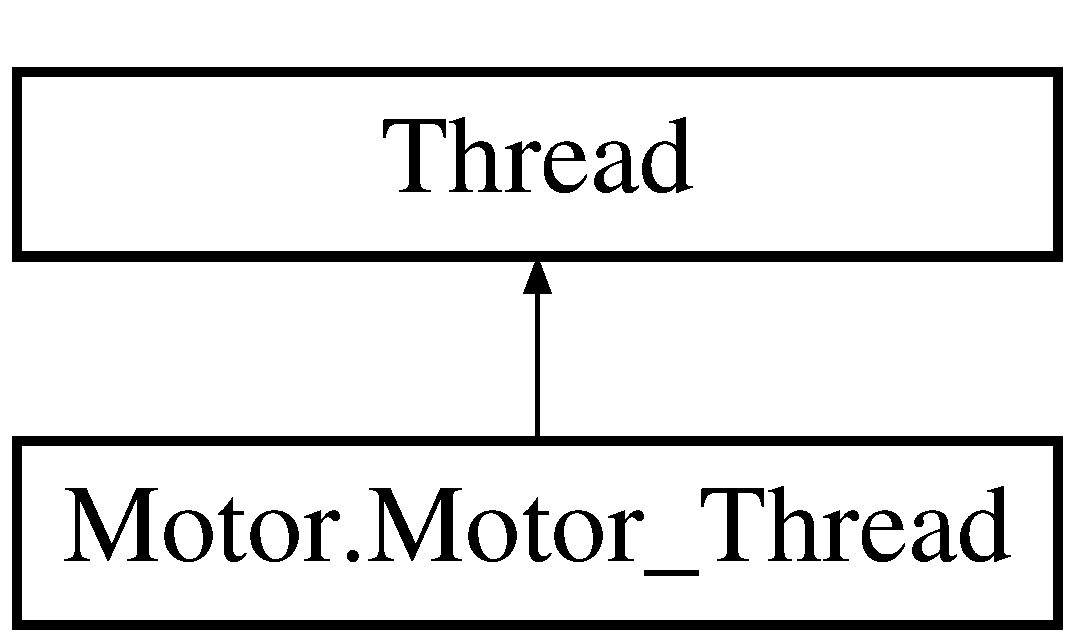
\includegraphics[height=2.000000cm]{class_motor_1_1_motor___thread}
\end{center}
\end{figure}
\subsection*{Public Member Functions}
\begin{DoxyCompactItemize}
\item 
def \mbox{\hyperlink{class_motor_1_1_motor___thread_a5610243ba8010e6b71669361f8d9f005}{\+\_\+\+\_\+init\+\_\+\+\_\+}} (self, \mbox{\hyperlink{class_motor_1_1_motor___thread_a67c6a328eb97c9a8ea0524b43a29f15c}{motor}})
\item 
def \mbox{\hyperlink{class_motor_1_1_motor___thread_a940954129ae966e7250b3335d4a78f1d}{run}} (self)
\end{DoxyCompactItemize}
\subsection*{Public Attributes}
\begin{DoxyCompactItemize}
\item 
\mbox{\hyperlink{class_motor_1_1_motor___thread_a67c6a328eb97c9a8ea0524b43a29f15c}{motor}}
\end{DoxyCompactItemize}


\subsection{Detailed Description}
\begin{DoxyVerb}Thread for the motor, emulates PWM to control it
\end{DoxyVerb}
 

\subsection{Constructor \& Destructor Documentation}
\mbox{\Hypertarget{class_motor_1_1_motor___thread_a5610243ba8010e6b71669361f8d9f005}\label{class_motor_1_1_motor___thread_a5610243ba8010e6b71669361f8d9f005}} 
\index{Motor\+::\+Motor\+\_\+\+Thread@{Motor\+::\+Motor\+\_\+\+Thread}!\+\_\+\+\_\+init\+\_\+\+\_\+@{\+\_\+\+\_\+init\+\_\+\+\_\+}}
\index{\+\_\+\+\_\+init\+\_\+\+\_\+@{\+\_\+\+\_\+init\+\_\+\+\_\+}!Motor\+::\+Motor\+\_\+\+Thread@{Motor\+::\+Motor\+\_\+\+Thread}}
\subsubsection{\texorpdfstring{\+\_\+\+\_\+init\+\_\+\+\_\+()}{\_\_init\_\_()}}
{\footnotesize\ttfamily def Motor.\+Motor\+\_\+\+Thread.\+\_\+\+\_\+init\+\_\+\+\_\+ (\begin{DoxyParamCaption}\item[{}]{self,  }\item[{}]{motor }\end{DoxyParamCaption})}



\subsection{Member Function Documentation}
\mbox{\Hypertarget{class_motor_1_1_motor___thread_a940954129ae966e7250b3335d4a78f1d}\label{class_motor_1_1_motor___thread_a940954129ae966e7250b3335d4a78f1d}} 
\index{Motor\+::\+Motor\+\_\+\+Thread@{Motor\+::\+Motor\+\_\+\+Thread}!run@{run}}
\index{run@{run}!Motor\+::\+Motor\+\_\+\+Thread@{Motor\+::\+Motor\+\_\+\+Thread}}
\subsubsection{\texorpdfstring{run()}{run()}}
{\footnotesize\ttfamily def Motor.\+Motor\+\_\+\+Thread.\+run (\begin{DoxyParamCaption}\item[{}]{self }\end{DoxyParamCaption})}



\subsection{Member Data Documentation}
\mbox{\Hypertarget{class_motor_1_1_motor___thread_a67c6a328eb97c9a8ea0524b43a29f15c}\label{class_motor_1_1_motor___thread_a67c6a328eb97c9a8ea0524b43a29f15c}} 
\index{Motor\+::\+Motor\+\_\+\+Thread@{Motor\+::\+Motor\+\_\+\+Thread}!motor@{motor}}
\index{motor@{motor}!Motor\+::\+Motor\+\_\+\+Thread@{Motor\+::\+Motor\+\_\+\+Thread}}
\subsubsection{\texorpdfstring{motor}{motor}}
{\footnotesize\ttfamily Motor.\+Motor\+\_\+\+Thread.\+motor}



The documentation for this class was generated from the following file\+:\begin{DoxyCompactItemize}
\item 
\mbox{\hyperlink{_motor_8py}{Motor.\+py}}\end{DoxyCompactItemize}

\hypertarget{class_robot_1_1_robot}{}\section{Robot.\+Robot Class Reference}
\label{class_robot_1_1_robot}\index{Robot.\+Robot@{Robot.\+Robot}}
\subsection*{Public Member Functions}
\begin{DoxyCompactItemize}
\item 
def \mbox{\hyperlink{class_robot_1_1_robot_a40c577b70d0dc59d0ea36c4418b4ebb8}{\+\_\+\+\_\+init\+\_\+\+\_\+}} (self, \mbox{\hyperlink{class_robot_1_1_robot_ac0e3d996cf1764a2b968186444554312}{wheels}}, \mbox{\hyperlink{class_robot_1_1_robot_a0d2df6b5b1ee9236e08f51468a22398d}{sensor\+\_\+vals}})
\item 
def \mbox{\hyperlink{class_robot_1_1_robot_ab1a6040ab6b4bde8fd8230b6f84cd8c8}{move\+\_\+forward}} (self, speed, duration)
\item 
def \mbox{\hyperlink{class_robot_1_1_robot_a4d9a177a012a52f6baee9c9dd7cb200b}{move\+\_\+backward}} (self, speed, duration)
\item 
def \mbox{\hyperlink{class_robot_1_1_robot_aeb19d8722b14e591d980f44887f5430b}{turn\+\_\+left}} (self, speed, duration)
\item 
def \mbox{\hyperlink{class_robot_1_1_robot_afd3797d558dd232b5c57ff1d2997024c}{turn\+\_\+right}} (self, speed, duration)
\item 
def \mbox{\hyperlink{class_robot_1_1_robot_a626830c7b3379821e487f14f44fe233d}{get\+\_\+sensor\+\_\+vals}} (self)
\end{DoxyCompactItemize}
\subsection*{Public Attributes}
\begin{DoxyCompactItemize}
\item 
\mbox{\hyperlink{class_robot_1_1_robot_ac0e3d996cf1764a2b968186444554312}{wheels}}
\item 
\mbox{\hyperlink{class_robot_1_1_robot_a0d2df6b5b1ee9236e08f51468a22398d}{sensor\+\_\+vals}}
\end{DoxyCompactItemize}


\subsection{Detailed Description}
\begin{DoxyVerb}Wrapper around the whole system.
The Robot object is interacted with which in turn interacts with the sub components
\end{DoxyVerb}
 

\subsection{Constructor \& Destructor Documentation}
\mbox{\Hypertarget{class_robot_1_1_robot_a40c577b70d0dc59d0ea36c4418b4ebb8}\label{class_robot_1_1_robot_a40c577b70d0dc59d0ea36c4418b4ebb8}} 
\index{Robot\+::\+Robot@{Robot\+::\+Robot}!\+\_\+\+\_\+init\+\_\+\+\_\+@{\+\_\+\+\_\+init\+\_\+\+\_\+}}
\index{\+\_\+\+\_\+init\+\_\+\+\_\+@{\+\_\+\+\_\+init\+\_\+\+\_\+}!Robot\+::\+Robot@{Robot\+::\+Robot}}
\subsubsection{\texorpdfstring{\+\_\+\+\_\+init\+\_\+\+\_\+()}{\_\_init\_\_()}}
{\footnotesize\ttfamily def Robot.\+Robot.\+\_\+\+\_\+init\+\_\+\+\_\+ (\begin{DoxyParamCaption}\item[{}]{self,  }\item[{}]{wheels,  }\item[{}]{sensor\+\_\+vals }\end{DoxyParamCaption})}



\subsection{Member Function Documentation}
\mbox{\Hypertarget{class_robot_1_1_robot_a626830c7b3379821e487f14f44fe233d}\label{class_robot_1_1_robot_a626830c7b3379821e487f14f44fe233d}} 
\index{Robot\+::\+Robot@{Robot\+::\+Robot}!get\+\_\+sensor\+\_\+vals@{get\+\_\+sensor\+\_\+vals}}
\index{get\+\_\+sensor\+\_\+vals@{get\+\_\+sensor\+\_\+vals}!Robot\+::\+Robot@{Robot\+::\+Robot}}
\subsubsection{\texorpdfstring{get\+\_\+sensor\+\_\+vals()}{get\_sensor\_vals()}}
{\footnotesize\ttfamily def Robot.\+Robot.\+get\+\_\+sensor\+\_\+vals (\begin{DoxyParamCaption}\item[{}]{self }\end{DoxyParamCaption})}

\mbox{\Hypertarget{class_robot_1_1_robot_a4d9a177a012a52f6baee9c9dd7cb200b}\label{class_robot_1_1_robot_a4d9a177a012a52f6baee9c9dd7cb200b}} 
\index{Robot\+::\+Robot@{Robot\+::\+Robot}!move\+\_\+backward@{move\+\_\+backward}}
\index{move\+\_\+backward@{move\+\_\+backward}!Robot\+::\+Robot@{Robot\+::\+Robot}}
\subsubsection{\texorpdfstring{move\+\_\+backward()}{move\_backward()}}
{\footnotesize\ttfamily def Robot.\+Robot.\+move\+\_\+backward (\begin{DoxyParamCaption}\item[{}]{self,  }\item[{}]{speed,  }\item[{}]{duration }\end{DoxyParamCaption})}

\mbox{\Hypertarget{class_robot_1_1_robot_ab1a6040ab6b4bde8fd8230b6f84cd8c8}\label{class_robot_1_1_robot_ab1a6040ab6b4bde8fd8230b6f84cd8c8}} 
\index{Robot\+::\+Robot@{Robot\+::\+Robot}!move\+\_\+forward@{move\+\_\+forward}}
\index{move\+\_\+forward@{move\+\_\+forward}!Robot\+::\+Robot@{Robot\+::\+Robot}}
\subsubsection{\texorpdfstring{move\+\_\+forward()}{move\_forward()}}
{\footnotesize\ttfamily def Robot.\+Robot.\+move\+\_\+forward (\begin{DoxyParamCaption}\item[{}]{self,  }\item[{}]{speed,  }\item[{}]{duration }\end{DoxyParamCaption})}

\mbox{\Hypertarget{class_robot_1_1_robot_aeb19d8722b14e591d980f44887f5430b}\label{class_robot_1_1_robot_aeb19d8722b14e591d980f44887f5430b}} 
\index{Robot\+::\+Robot@{Robot\+::\+Robot}!turn\+\_\+left@{turn\+\_\+left}}
\index{turn\+\_\+left@{turn\+\_\+left}!Robot\+::\+Robot@{Robot\+::\+Robot}}
\subsubsection{\texorpdfstring{turn\+\_\+left()}{turn\_left()}}
{\footnotesize\ttfamily def Robot.\+Robot.\+turn\+\_\+left (\begin{DoxyParamCaption}\item[{}]{self,  }\item[{}]{speed,  }\item[{}]{duration }\end{DoxyParamCaption})}

\mbox{\Hypertarget{class_robot_1_1_robot_afd3797d558dd232b5c57ff1d2997024c}\label{class_robot_1_1_robot_afd3797d558dd232b5c57ff1d2997024c}} 
\index{Robot\+::\+Robot@{Robot\+::\+Robot}!turn\+\_\+right@{turn\+\_\+right}}
\index{turn\+\_\+right@{turn\+\_\+right}!Robot\+::\+Robot@{Robot\+::\+Robot}}
\subsubsection{\texorpdfstring{turn\+\_\+right()}{turn\_right()}}
{\footnotesize\ttfamily def Robot.\+Robot.\+turn\+\_\+right (\begin{DoxyParamCaption}\item[{}]{self,  }\item[{}]{speed,  }\item[{}]{duration }\end{DoxyParamCaption})}



\subsection{Member Data Documentation}
\mbox{\Hypertarget{class_robot_1_1_robot_a0d2df6b5b1ee9236e08f51468a22398d}\label{class_robot_1_1_robot_a0d2df6b5b1ee9236e08f51468a22398d}} 
\index{Robot\+::\+Robot@{Robot\+::\+Robot}!sensor\+\_\+vals@{sensor\+\_\+vals}}
\index{sensor\+\_\+vals@{sensor\+\_\+vals}!Robot\+::\+Robot@{Robot\+::\+Robot}}
\subsubsection{\texorpdfstring{sensor\+\_\+vals}{sensor\_vals}}
{\footnotesize\ttfamily Robot.\+Robot.\+sensor\+\_\+vals}

\mbox{\Hypertarget{class_robot_1_1_robot_ac0e3d996cf1764a2b968186444554312}\label{class_robot_1_1_robot_ac0e3d996cf1764a2b968186444554312}} 
\index{Robot\+::\+Robot@{Robot\+::\+Robot}!wheels@{wheels}}
\index{wheels@{wheels}!Robot\+::\+Robot@{Robot\+::\+Robot}}
\subsubsection{\texorpdfstring{wheels}{wheels}}
{\footnotesize\ttfamily Robot.\+Robot.\+wheels}



The documentation for this class was generated from the following file\+:\begin{DoxyCompactItemize}
\item 
\mbox{\hyperlink{_robot_8py}{Robot.\+py}}\end{DoxyCompactItemize}

\hypertarget{class_ultrasonic__sensors_1_1_ultrasonic___sensor}{}\section{Ultrasonic\+\_\+sensors.\+Ultrasonic\+\_\+\+Sensor Class Reference}
\label{class_ultrasonic__sensors_1_1_ultrasonic___sensor}\index{Ultrasonic\+\_\+sensors.\+Ultrasonic\+\_\+\+Sensor@{Ultrasonic\+\_\+sensors.\+Ultrasonic\+\_\+\+Sensor}}
\subsection*{Public Member Functions}
\begin{DoxyCompactItemize}
\item 
def \mbox{\hyperlink{class_ultrasonic__sensors_1_1_ultrasonic___sensor_a90b69a01f5b8060357bb1694ac9ad10e}{\+\_\+\+\_\+init\+\_\+\+\_\+}} (self, \mbox{\hyperlink{class_ultrasonic__sensors_1_1_ultrasonic___sensor_a5bfbddc32c4566f14e0a10f9c1a05c1e}{ID}}, \mbox{\hyperlink{class_ultrasonic__sensors_1_1_ultrasonic___sensor_a72e525e29f7c8641247068f2daae2632}{trig}}, \mbox{\hyperlink{class_ultrasonic__sensors_1_1_ultrasonic___sensor_add8bcdab8946934ae7d20f2173bd9b9d}{echo}}, \mbox{\hyperlink{class_ultrasonic__sensors_1_1_ultrasonic___sensor_a3ab17c4f96a9961e835e447227a29399}{threshold}})
\item 
def \mbox{\hyperlink{class_ultrasonic__sensors_1_1_ultrasonic___sensor_a0fd98fc2563beaabadeafa073220a367}{get\+\_\+distance}} (self)
\item 
def \mbox{\hyperlink{class_ultrasonic__sensors_1_1_ultrasonic___sensor_ad081ca76bfd75937c4fc973552bf1389}{get\+\_\+info}} (self)
\end{DoxyCompactItemize}
\subsection*{Public Attributes}
\begin{DoxyCompactItemize}
\item 
\mbox{\hyperlink{class_ultrasonic__sensors_1_1_ultrasonic___sensor_a5bfbddc32c4566f14e0a10f9c1a05c1e}{ID}}
\item 
\mbox{\hyperlink{class_ultrasonic__sensors_1_1_ultrasonic___sensor_a72e525e29f7c8641247068f2daae2632}{trig}}
\item 
\mbox{\hyperlink{class_ultrasonic__sensors_1_1_ultrasonic___sensor_add8bcdab8946934ae7d20f2173bd9b9d}{echo}}
\item 
\mbox{\hyperlink{class_ultrasonic__sensors_1_1_ultrasonic___sensor_a3ab17c4f96a9961e835e447227a29399}{threshold}}
\end{DoxyCompactItemize}


\subsection{Constructor \& Destructor Documentation}
\mbox{\Hypertarget{class_ultrasonic__sensors_1_1_ultrasonic___sensor_a90b69a01f5b8060357bb1694ac9ad10e}\label{class_ultrasonic__sensors_1_1_ultrasonic___sensor_a90b69a01f5b8060357bb1694ac9ad10e}} 
\index{Ultrasonic\+\_\+sensors\+::\+Ultrasonic\+\_\+\+Sensor@{Ultrasonic\+\_\+sensors\+::\+Ultrasonic\+\_\+\+Sensor}!\+\_\+\+\_\+init\+\_\+\+\_\+@{\+\_\+\+\_\+init\+\_\+\+\_\+}}
\index{\+\_\+\+\_\+init\+\_\+\+\_\+@{\+\_\+\+\_\+init\+\_\+\+\_\+}!Ultrasonic\+\_\+sensors\+::\+Ultrasonic\+\_\+\+Sensor@{Ultrasonic\+\_\+sensors\+::\+Ultrasonic\+\_\+\+Sensor}}
\subsubsection{\texorpdfstring{\+\_\+\+\_\+init\+\_\+\+\_\+()}{\_\_init\_\_()}}
{\footnotesize\ttfamily def Ultrasonic\+\_\+sensors.\+Ultrasonic\+\_\+\+Sensor.\+\_\+\+\_\+init\+\_\+\+\_\+ (\begin{DoxyParamCaption}\item[{}]{self,  }\item[{}]{ID,  }\item[{}]{trig,  }\item[{}]{echo,  }\item[{}]{threshold }\end{DoxyParamCaption})}



\subsection{Member Function Documentation}
\mbox{\Hypertarget{class_ultrasonic__sensors_1_1_ultrasonic___sensor_a0fd98fc2563beaabadeafa073220a367}\label{class_ultrasonic__sensors_1_1_ultrasonic___sensor_a0fd98fc2563beaabadeafa073220a367}} 
\index{Ultrasonic\+\_\+sensors\+::\+Ultrasonic\+\_\+\+Sensor@{Ultrasonic\+\_\+sensors\+::\+Ultrasonic\+\_\+\+Sensor}!get\+\_\+distance@{get\+\_\+distance}}
\index{get\+\_\+distance@{get\+\_\+distance}!Ultrasonic\+\_\+sensors\+::\+Ultrasonic\+\_\+\+Sensor@{Ultrasonic\+\_\+sensors\+::\+Ultrasonic\+\_\+\+Sensor}}
\subsubsection{\texorpdfstring{get\+\_\+distance()}{get\_distance()}}
{\footnotesize\ttfamily def Ultrasonic\+\_\+sensors.\+Ultrasonic\+\_\+\+Sensor.\+get\+\_\+distance (\begin{DoxyParamCaption}\item[{}]{self }\end{DoxyParamCaption})}

\mbox{\Hypertarget{class_ultrasonic__sensors_1_1_ultrasonic___sensor_ad081ca76bfd75937c4fc973552bf1389}\label{class_ultrasonic__sensors_1_1_ultrasonic___sensor_ad081ca76bfd75937c4fc973552bf1389}} 
\index{Ultrasonic\+\_\+sensors\+::\+Ultrasonic\+\_\+\+Sensor@{Ultrasonic\+\_\+sensors\+::\+Ultrasonic\+\_\+\+Sensor}!get\+\_\+info@{get\+\_\+info}}
\index{get\+\_\+info@{get\+\_\+info}!Ultrasonic\+\_\+sensors\+::\+Ultrasonic\+\_\+\+Sensor@{Ultrasonic\+\_\+sensors\+::\+Ultrasonic\+\_\+\+Sensor}}
\subsubsection{\texorpdfstring{get\+\_\+info()}{get\_info()}}
{\footnotesize\ttfamily def Ultrasonic\+\_\+sensors.\+Ultrasonic\+\_\+\+Sensor.\+get\+\_\+info (\begin{DoxyParamCaption}\item[{}]{self }\end{DoxyParamCaption})}



\subsection{Member Data Documentation}
\mbox{\Hypertarget{class_ultrasonic__sensors_1_1_ultrasonic___sensor_add8bcdab8946934ae7d20f2173bd9b9d}\label{class_ultrasonic__sensors_1_1_ultrasonic___sensor_add8bcdab8946934ae7d20f2173bd9b9d}} 
\index{Ultrasonic\+\_\+sensors\+::\+Ultrasonic\+\_\+\+Sensor@{Ultrasonic\+\_\+sensors\+::\+Ultrasonic\+\_\+\+Sensor}!echo@{echo}}
\index{echo@{echo}!Ultrasonic\+\_\+sensors\+::\+Ultrasonic\+\_\+\+Sensor@{Ultrasonic\+\_\+sensors\+::\+Ultrasonic\+\_\+\+Sensor}}
\subsubsection{\texorpdfstring{echo}{echo}}
{\footnotesize\ttfamily Ultrasonic\+\_\+sensors.\+Ultrasonic\+\_\+\+Sensor.\+echo}

\mbox{\Hypertarget{class_ultrasonic__sensors_1_1_ultrasonic___sensor_a5bfbddc32c4566f14e0a10f9c1a05c1e}\label{class_ultrasonic__sensors_1_1_ultrasonic___sensor_a5bfbddc32c4566f14e0a10f9c1a05c1e}} 
\index{Ultrasonic\+\_\+sensors\+::\+Ultrasonic\+\_\+\+Sensor@{Ultrasonic\+\_\+sensors\+::\+Ultrasonic\+\_\+\+Sensor}!ID@{ID}}
\index{ID@{ID}!Ultrasonic\+\_\+sensors\+::\+Ultrasonic\+\_\+\+Sensor@{Ultrasonic\+\_\+sensors\+::\+Ultrasonic\+\_\+\+Sensor}}
\subsubsection{\texorpdfstring{ID}{ID}}
{\footnotesize\ttfamily Ultrasonic\+\_\+sensors.\+Ultrasonic\+\_\+\+Sensor.\+ID}

\mbox{\Hypertarget{class_ultrasonic__sensors_1_1_ultrasonic___sensor_a3ab17c4f96a9961e835e447227a29399}\label{class_ultrasonic__sensors_1_1_ultrasonic___sensor_a3ab17c4f96a9961e835e447227a29399}} 
\index{Ultrasonic\+\_\+sensors\+::\+Ultrasonic\+\_\+\+Sensor@{Ultrasonic\+\_\+sensors\+::\+Ultrasonic\+\_\+\+Sensor}!threshold@{threshold}}
\index{threshold@{threshold}!Ultrasonic\+\_\+sensors\+::\+Ultrasonic\+\_\+\+Sensor@{Ultrasonic\+\_\+sensors\+::\+Ultrasonic\+\_\+\+Sensor}}
\subsubsection{\texorpdfstring{threshold}{threshold}}
{\footnotesize\ttfamily Ultrasonic\+\_\+sensors.\+Ultrasonic\+\_\+\+Sensor.\+threshold}

\mbox{\Hypertarget{class_ultrasonic__sensors_1_1_ultrasonic___sensor_a72e525e29f7c8641247068f2daae2632}\label{class_ultrasonic__sensors_1_1_ultrasonic___sensor_a72e525e29f7c8641247068f2daae2632}} 
\index{Ultrasonic\+\_\+sensors\+::\+Ultrasonic\+\_\+\+Sensor@{Ultrasonic\+\_\+sensors\+::\+Ultrasonic\+\_\+\+Sensor}!trig@{trig}}
\index{trig@{trig}!Ultrasonic\+\_\+sensors\+::\+Ultrasonic\+\_\+\+Sensor@{Ultrasonic\+\_\+sensors\+::\+Ultrasonic\+\_\+\+Sensor}}
\subsubsection{\texorpdfstring{trig}{trig}}
{\footnotesize\ttfamily Ultrasonic\+\_\+sensors.\+Ultrasonic\+\_\+\+Sensor.\+trig}



The documentation for this class was generated from the following file\+:\begin{DoxyCompactItemize}
\item 
\mbox{\hyperlink{_ultrasonic__sensors_8py}{Ultrasonic\+\_\+sensors.\+py}}\end{DoxyCompactItemize}

\hypertarget{class_ultrasonic__sensors_1_1_ultrasonic___sensor___thread}{}\section{Ultrasonic\+\_\+sensors.\+Ultrasonic\+\_\+\+Sensor\+\_\+\+Thread Class Reference}
\label{class_ultrasonic__sensors_1_1_ultrasonic___sensor___thread}\index{Ultrasonic\+\_\+sensors.\+Ultrasonic\+\_\+\+Sensor\+\_\+\+Thread@{Ultrasonic\+\_\+sensors.\+Ultrasonic\+\_\+\+Sensor\+\_\+\+Thread}}
Inheritance diagram for Ultrasonic\+\_\+sensors.\+Ultrasonic\+\_\+\+Sensor\+\_\+\+Thread\+:\begin{figure}[H]
\begin{center}
\leavevmode
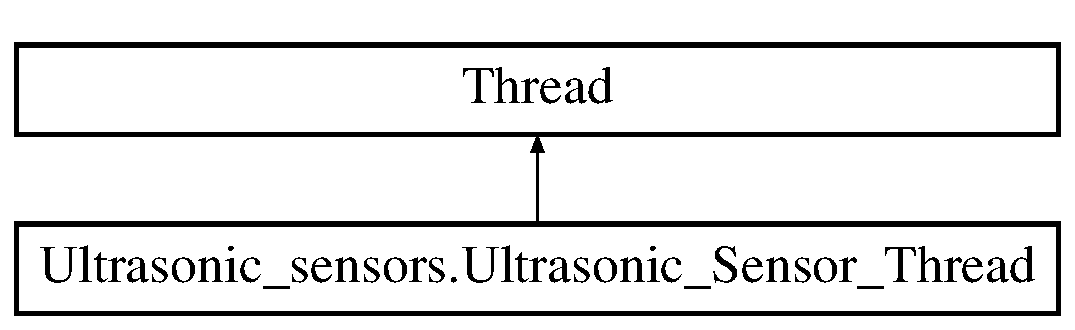
\includegraphics[height=2.000000cm]{class_ultrasonic__sensors_1_1_ultrasonic___sensor___thread}
\end{center}
\end{figure}
\subsection*{Public Member Functions}
\begin{DoxyCompactItemize}
\item 
def \mbox{\hyperlink{class_ultrasonic__sensors_1_1_ultrasonic___sensor___thread_a06d1bfe89cff77467a2dca1e4b89cb91}{\+\_\+\+\_\+init\+\_\+\+\_\+}} (self, \mbox{\hyperlink{class_ultrasonic__sensors_1_1_ultrasonic___sensor___thread_a2cb18fd9999c266a7011d3ab17e09c1a}{sensor}}, \mbox{\hyperlink{class_ultrasonic__sensors_1_1_ultrasonic___sensor___thread_aa854d163320bedc21a2db58848afd51c}{sensor\+\_\+values}}, \mbox{\hyperlink{class_ultrasonic__sensors_1_1_ultrasonic___sensor___thread_a2cb683e88f0562d6fed96642ab157a38}{rate}})
\item 
def \mbox{\hyperlink{class_ultrasonic__sensors_1_1_ultrasonic___sensor___thread_ad074f29246b4db6af7b2488ec7d4b276}{run}} (self)
\end{DoxyCompactItemize}
\subsection*{Public Attributes}
\begin{DoxyCompactItemize}
\item 
\mbox{\hyperlink{class_ultrasonic__sensors_1_1_ultrasonic___sensor___thread_a2cb18fd9999c266a7011d3ab17e09c1a}{sensor}}
\item 
\mbox{\hyperlink{class_ultrasonic__sensors_1_1_ultrasonic___sensor___thread_aa854d163320bedc21a2db58848afd51c}{sensor\+\_\+values}}
\item 
\mbox{\hyperlink{class_ultrasonic__sensors_1_1_ultrasonic___sensor___thread_a2cb683e88f0562d6fed96642ab157a38}{rate}}
\end{DoxyCompactItemize}


\subsection{Constructor \& Destructor Documentation}
\mbox{\Hypertarget{class_ultrasonic__sensors_1_1_ultrasonic___sensor___thread_a06d1bfe89cff77467a2dca1e4b89cb91}\label{class_ultrasonic__sensors_1_1_ultrasonic___sensor___thread_a06d1bfe89cff77467a2dca1e4b89cb91}} 
\index{Ultrasonic\+\_\+sensors\+::\+Ultrasonic\+\_\+\+Sensor\+\_\+\+Thread@{Ultrasonic\+\_\+sensors\+::\+Ultrasonic\+\_\+\+Sensor\+\_\+\+Thread}!\+\_\+\+\_\+init\+\_\+\+\_\+@{\+\_\+\+\_\+init\+\_\+\+\_\+}}
\index{\+\_\+\+\_\+init\+\_\+\+\_\+@{\+\_\+\+\_\+init\+\_\+\+\_\+}!Ultrasonic\+\_\+sensors\+::\+Ultrasonic\+\_\+\+Sensor\+\_\+\+Thread@{Ultrasonic\+\_\+sensors\+::\+Ultrasonic\+\_\+\+Sensor\+\_\+\+Thread}}
\subsubsection{\texorpdfstring{\+\_\+\+\_\+init\+\_\+\+\_\+()}{\_\_init\_\_()}}
{\footnotesize\ttfamily def Ultrasonic\+\_\+sensors.\+Ultrasonic\+\_\+\+Sensor\+\_\+\+Thread.\+\_\+\+\_\+init\+\_\+\+\_\+ (\begin{DoxyParamCaption}\item[{}]{self,  }\item[{}]{sensor,  }\item[{}]{sensor\+\_\+values,  }\item[{}]{rate }\end{DoxyParamCaption})}



\subsection{Member Function Documentation}
\mbox{\Hypertarget{class_ultrasonic__sensors_1_1_ultrasonic___sensor___thread_ad074f29246b4db6af7b2488ec7d4b276}\label{class_ultrasonic__sensors_1_1_ultrasonic___sensor___thread_ad074f29246b4db6af7b2488ec7d4b276}} 
\index{Ultrasonic\+\_\+sensors\+::\+Ultrasonic\+\_\+\+Sensor\+\_\+\+Thread@{Ultrasonic\+\_\+sensors\+::\+Ultrasonic\+\_\+\+Sensor\+\_\+\+Thread}!run@{run}}
\index{run@{run}!Ultrasonic\+\_\+sensors\+::\+Ultrasonic\+\_\+\+Sensor\+\_\+\+Thread@{Ultrasonic\+\_\+sensors\+::\+Ultrasonic\+\_\+\+Sensor\+\_\+\+Thread}}
\subsubsection{\texorpdfstring{run()}{run()}}
{\footnotesize\ttfamily def Ultrasonic\+\_\+sensors.\+Ultrasonic\+\_\+\+Sensor\+\_\+\+Thread.\+run (\begin{DoxyParamCaption}\item[{}]{self }\end{DoxyParamCaption})}



\subsection{Member Data Documentation}
\mbox{\Hypertarget{class_ultrasonic__sensors_1_1_ultrasonic___sensor___thread_a2cb683e88f0562d6fed96642ab157a38}\label{class_ultrasonic__sensors_1_1_ultrasonic___sensor___thread_a2cb683e88f0562d6fed96642ab157a38}} 
\index{Ultrasonic\+\_\+sensors\+::\+Ultrasonic\+\_\+\+Sensor\+\_\+\+Thread@{Ultrasonic\+\_\+sensors\+::\+Ultrasonic\+\_\+\+Sensor\+\_\+\+Thread}!rate@{rate}}
\index{rate@{rate}!Ultrasonic\+\_\+sensors\+::\+Ultrasonic\+\_\+\+Sensor\+\_\+\+Thread@{Ultrasonic\+\_\+sensors\+::\+Ultrasonic\+\_\+\+Sensor\+\_\+\+Thread}}
\subsubsection{\texorpdfstring{rate}{rate}}
{\footnotesize\ttfamily Ultrasonic\+\_\+sensors.\+Ultrasonic\+\_\+\+Sensor\+\_\+\+Thread.\+rate}

\mbox{\Hypertarget{class_ultrasonic__sensors_1_1_ultrasonic___sensor___thread_a2cb18fd9999c266a7011d3ab17e09c1a}\label{class_ultrasonic__sensors_1_1_ultrasonic___sensor___thread_a2cb18fd9999c266a7011d3ab17e09c1a}} 
\index{Ultrasonic\+\_\+sensors\+::\+Ultrasonic\+\_\+\+Sensor\+\_\+\+Thread@{Ultrasonic\+\_\+sensors\+::\+Ultrasonic\+\_\+\+Sensor\+\_\+\+Thread}!sensor@{sensor}}
\index{sensor@{sensor}!Ultrasonic\+\_\+sensors\+::\+Ultrasonic\+\_\+\+Sensor\+\_\+\+Thread@{Ultrasonic\+\_\+sensors\+::\+Ultrasonic\+\_\+\+Sensor\+\_\+\+Thread}}
\subsubsection{\texorpdfstring{sensor}{sensor}}
{\footnotesize\ttfamily Ultrasonic\+\_\+sensors.\+Ultrasonic\+\_\+\+Sensor\+\_\+\+Thread.\+sensor}

\mbox{\Hypertarget{class_ultrasonic__sensors_1_1_ultrasonic___sensor___thread_aa854d163320bedc21a2db58848afd51c}\label{class_ultrasonic__sensors_1_1_ultrasonic___sensor___thread_aa854d163320bedc21a2db58848afd51c}} 
\index{Ultrasonic\+\_\+sensors\+::\+Ultrasonic\+\_\+\+Sensor\+\_\+\+Thread@{Ultrasonic\+\_\+sensors\+::\+Ultrasonic\+\_\+\+Sensor\+\_\+\+Thread}!sensor\+\_\+values@{sensor\+\_\+values}}
\index{sensor\+\_\+values@{sensor\+\_\+values}!Ultrasonic\+\_\+sensors\+::\+Ultrasonic\+\_\+\+Sensor\+\_\+\+Thread@{Ultrasonic\+\_\+sensors\+::\+Ultrasonic\+\_\+\+Sensor\+\_\+\+Thread}}
\subsubsection{\texorpdfstring{sensor\+\_\+values}{sensor\_values}}
{\footnotesize\ttfamily Ultrasonic\+\_\+sensors.\+Ultrasonic\+\_\+\+Sensor\+\_\+\+Thread.\+sensor\+\_\+values}



The documentation for this class was generated from the following file\+:\begin{DoxyCompactItemize}
\item 
\mbox{\hyperlink{_ultrasonic__sensors_8py}{Ultrasonic\+\_\+sensors.\+py}}\end{DoxyCompactItemize}

\hypertarget{class_wheels_1_1_wheels}{}\section{Wheels.\+Wheels Class Reference}
\label{class_wheels_1_1_wheels}\index{Wheels.\+Wheels@{Wheels.\+Wheels}}
\subsection*{Public Member Functions}
\begin{DoxyCompactItemize}
\item 
def \mbox{\hyperlink{class_wheels_1_1_wheels_afab89c68fc8a1f8aeb8b932d97cf7999}{\+\_\+\+\_\+init\+\_\+\+\_\+}} (self, \mbox{\hyperlink{class_wheels_1_1_wheels_a47e8526b08d3a33a7c03524bde27b659}{left}}, \mbox{\hyperlink{class_wheels_1_1_wheels_ac10912e5e2dc289a21f222787c4e0f98}{right}})
\item 
def \mbox{\hyperlink{class_wheels_1_1_wheels_a71354795014dc6c28125b1c86666b8b4}{turn\+\_\+left}} (self, speed, duration)
\item 
def \mbox{\hyperlink{class_wheels_1_1_wheels_a325e09d58c40e88dbe2d1fda1295b26f}{turn\+\_\+right}} (self, speed, duration)
\item 
def \mbox{\hyperlink{class_wheels_1_1_wheels_a30bd7a5a1d962cad87a27409d1afbcd4}{forward}} (self, speed, duration)
\item 
def \mbox{\hyperlink{class_wheels_1_1_wheels_ae243add297cf9719249b658818c9a229}{reverse}} (self, speed, duration)
\end{DoxyCompactItemize}
\subsection*{Public Attributes}
\begin{DoxyCompactItemize}
\item 
\mbox{\hyperlink{class_wheels_1_1_wheels_a47e8526b08d3a33a7c03524bde27b659}{left}}
\item 
\mbox{\hyperlink{class_wheels_1_1_wheels_ac10912e5e2dc289a21f222787c4e0f98}{right}}
\end{DoxyCompactItemize}


\subsection{Detailed Description}
\begin{DoxyVerb}A wrapper around two motors
\end{DoxyVerb}
 

\subsection{Constructor \& Destructor Documentation}
\mbox{\Hypertarget{class_wheels_1_1_wheels_afab89c68fc8a1f8aeb8b932d97cf7999}\label{class_wheels_1_1_wheels_afab89c68fc8a1f8aeb8b932d97cf7999}} 
\index{Wheels\+::\+Wheels@{Wheels\+::\+Wheels}!\+\_\+\+\_\+init\+\_\+\+\_\+@{\+\_\+\+\_\+init\+\_\+\+\_\+}}
\index{\+\_\+\+\_\+init\+\_\+\+\_\+@{\+\_\+\+\_\+init\+\_\+\+\_\+}!Wheels\+::\+Wheels@{Wheels\+::\+Wheels}}
\subsubsection{\texorpdfstring{\+\_\+\+\_\+init\+\_\+\+\_\+()}{\_\_init\_\_()}}
{\footnotesize\ttfamily def Wheels.\+Wheels.\+\_\+\+\_\+init\+\_\+\+\_\+ (\begin{DoxyParamCaption}\item[{}]{self,  }\item[{}]{left,  }\item[{}]{right }\end{DoxyParamCaption})}



\subsection{Member Function Documentation}
\mbox{\Hypertarget{class_wheels_1_1_wheels_a30bd7a5a1d962cad87a27409d1afbcd4}\label{class_wheels_1_1_wheels_a30bd7a5a1d962cad87a27409d1afbcd4}} 
\index{Wheels\+::\+Wheels@{Wheels\+::\+Wheels}!forward@{forward}}
\index{forward@{forward}!Wheels\+::\+Wheels@{Wheels\+::\+Wheels}}
\subsubsection{\texorpdfstring{forward()}{forward()}}
{\footnotesize\ttfamily def Wheels.\+Wheels.\+forward (\begin{DoxyParamCaption}\item[{}]{self,  }\item[{}]{speed,  }\item[{}]{duration }\end{DoxyParamCaption})}

\mbox{\Hypertarget{class_wheels_1_1_wheels_ae243add297cf9719249b658818c9a229}\label{class_wheels_1_1_wheels_ae243add297cf9719249b658818c9a229}} 
\index{Wheels\+::\+Wheels@{Wheels\+::\+Wheels}!reverse@{reverse}}
\index{reverse@{reverse}!Wheels\+::\+Wheels@{Wheels\+::\+Wheels}}
\subsubsection{\texorpdfstring{reverse()}{reverse()}}
{\footnotesize\ttfamily def Wheels.\+Wheels.\+reverse (\begin{DoxyParamCaption}\item[{}]{self,  }\item[{}]{speed,  }\item[{}]{duration }\end{DoxyParamCaption})}

\mbox{\Hypertarget{class_wheels_1_1_wheels_a71354795014dc6c28125b1c86666b8b4}\label{class_wheels_1_1_wheels_a71354795014dc6c28125b1c86666b8b4}} 
\index{Wheels\+::\+Wheels@{Wheels\+::\+Wheels}!turn\+\_\+left@{turn\+\_\+left}}
\index{turn\+\_\+left@{turn\+\_\+left}!Wheels\+::\+Wheels@{Wheels\+::\+Wheels}}
\subsubsection{\texorpdfstring{turn\+\_\+left()}{turn\_left()}}
{\footnotesize\ttfamily def Wheels.\+Wheels.\+turn\+\_\+left (\begin{DoxyParamCaption}\item[{}]{self,  }\item[{}]{speed,  }\item[{}]{duration }\end{DoxyParamCaption})}

\mbox{\Hypertarget{class_wheels_1_1_wheels_a325e09d58c40e88dbe2d1fda1295b26f}\label{class_wheels_1_1_wheels_a325e09d58c40e88dbe2d1fda1295b26f}} 
\index{Wheels\+::\+Wheels@{Wheels\+::\+Wheels}!turn\+\_\+right@{turn\+\_\+right}}
\index{turn\+\_\+right@{turn\+\_\+right}!Wheels\+::\+Wheels@{Wheels\+::\+Wheels}}
\subsubsection{\texorpdfstring{turn\+\_\+right()}{turn\_right()}}
{\footnotesize\ttfamily def Wheels.\+Wheels.\+turn\+\_\+right (\begin{DoxyParamCaption}\item[{}]{self,  }\item[{}]{speed,  }\item[{}]{duration }\end{DoxyParamCaption})}



\subsection{Member Data Documentation}
\mbox{\Hypertarget{class_wheels_1_1_wheels_a47e8526b08d3a33a7c03524bde27b659}\label{class_wheels_1_1_wheels_a47e8526b08d3a33a7c03524bde27b659}} 
\index{Wheels\+::\+Wheels@{Wheels\+::\+Wheels}!left@{left}}
\index{left@{left}!Wheels\+::\+Wheels@{Wheels\+::\+Wheels}}
\subsubsection{\texorpdfstring{left}{left}}
{\footnotesize\ttfamily Wheels.\+Wheels.\+left}

\mbox{\Hypertarget{class_wheels_1_1_wheels_ac10912e5e2dc289a21f222787c4e0f98}\label{class_wheels_1_1_wheels_ac10912e5e2dc289a21f222787c4e0f98}} 
\index{Wheels\+::\+Wheels@{Wheels\+::\+Wheels}!right@{right}}
\index{right@{right}!Wheels\+::\+Wheels@{Wheels\+::\+Wheels}}
\subsubsection{\texorpdfstring{right}{right}}
{\footnotesize\ttfamily Wheels.\+Wheels.\+right}



The documentation for this class was generated from the following file\+:\begin{DoxyCompactItemize}
\item 
\mbox{\hyperlink{_wheels_8py}{Wheels.\+py}}\end{DoxyCompactItemize}

\chapter{File Documentation}
\hypertarget{_arm_8py}{}\section{Arm.\+py File Reference}
\label{_arm_8py}\index{Arm.\+py@{Arm.\+py}}
\subsection*{Classes}
\begin{DoxyCompactItemize}
\item 
class \mbox{\hyperlink{class_arm_1_1_arm}{Arm.\+Arm}}
\end{DoxyCompactItemize}
\subsection*{Namespaces}
\begin{DoxyCompactItemize}
\item 
 \mbox{\hyperlink{namespace_arm}{Arm}}
\end{DoxyCompactItemize}

\hypertarget{check__pins_8py}{}\section{check\+\_\+pins.\+py File Reference}
\label{check__pins_8py}\index{check\+\_\+pins.\+py@{check\+\_\+pins.\+py}}
\subsection*{Namespaces}
\begin{DoxyCompactItemize}
\item 
 \mbox{\hyperlink{namespacecheck__pins}{check\+\_\+pins}}
\end{DoxyCompactItemize}
\subsection*{Variables}
\begin{DoxyCompactItemize}
\item 
list \mbox{\hyperlink{namespacecheck__pins_ae7e56ca97a6e158edc4836330a89f5bb}{check\+\_\+pins.\+pins}} = \mbox{[}31, 33, 35, 37, 24, 26\mbox{]}
\end{DoxyCompactItemize}

\hypertarget{clean__up_8py}{}\section{clean\+\_\+up.\+py File Reference}
\label{clean__up_8py}\index{clean\+\_\+up.\+py@{clean\+\_\+up.\+py}}
\subsection*{Namespaces}
\begin{DoxyCompactItemize}
\item 
 \mbox{\hyperlink{namespaceclean__up}{clean\+\_\+up}}
\end{DoxyCompactItemize}

\hypertarget{controller_8py}{}\section{controller.\+py File Reference}
\label{controller_8py}\index{controller.\+py@{controller.\+py}}
\subsection*{Classes}
\begin{DoxyCompactItemize}
\item 
class \mbox{\hyperlink{classcontroller_1_1_control___thread}{controller.\+Control\+\_\+\+Thread}}
\end{DoxyCompactItemize}
\subsection*{Namespaces}
\begin{DoxyCompactItemize}
\item 
 \mbox{\hyperlink{namespacecontroller}{controller}}
\end{DoxyCompactItemize}
\subsection*{Variables}
\begin{DoxyCompactItemize}
\item 
\mbox{\hyperlink{namespacecontroller_accafb331d0342effadbbe3609c156598}{controller.\+left\+\_\+motor}} = \mbox{\hyperlink{class_motor_1_1_motor}{Motor.\+Motor}}(31, 33, 24)
\item 
\mbox{\hyperlink{namespacecontroller_a6d0f4d0ae0b1cc7e69b7094cec5d44e9}{controller.\+left\+\_\+motor\+\_\+t}} = \mbox{\hyperlink{class_motor_1_1_motor___thread}{Motor.\+Motor\+\_\+\+Thread}}(left\+\_\+motor)
\item 
\mbox{\hyperlink{namespacecontroller_a01c7aa0aed71e493785716166c882f4f}{controller.\+right\+\_\+motor}} = \mbox{\hyperlink{class_motor_1_1_motor}{Motor.\+Motor}}(35, 37, 26)
\item 
\mbox{\hyperlink{namespacecontroller_a6256e3281526776faed48e0dbfb596ec}{controller.\+right\+\_\+motor\+\_\+t}} = \mbox{\hyperlink{class_motor_1_1_motor___thread}{Motor.\+Motor\+\_\+\+Thread}}(right\+\_\+motor)
\item 
\mbox{\hyperlink{namespacecontroller_ac1696e3b9bdd35da786bc99515eee2b9}{controller.\+wheels}} = \mbox{\hyperlink{class_wheels_1_1_wheels}{Wheels.\+Wheels}}(left\+\_\+motor, right\+\_\+motor)
\item 
\mbox{\hyperlink{namespacecontroller_a189bd3b1eaf031673385cc627be55bee}{controller.\+sensor\+\_\+values}} = dict()
\item 
int \mbox{\hyperlink{namespacecontroller_a0875b114513cfcd900f5969aa48e9e91}{controller.\+rate}} = 1
\item 
\mbox{\hyperlink{namespacecontroller_a16bd60420374c0595e623e0f1706972a}{controller.\+robot}} = \mbox{\hyperlink{class_robot_1_1_robot}{Robot.\+Robot}}(wheels, sensor\+\_\+values)
\item 
\mbox{\hyperlink{namespacecontroller_a2445f7bc86ae8711053f9fe3bd4db5a9}{controller.\+c\+\_\+t}} = Control\+\_\+\+Thread(robot)
\end{DoxyCompactItemize}

\hypertarget{_motor_8py}{}\section{Motor.\+py File Reference}
\label{_motor_8py}\index{Motor.\+py@{Motor.\+py}}
\subsection*{Classes}
\begin{DoxyCompactItemize}
\item 
class \mbox{\hyperlink{class_motor_1_1_motor}{Motor.\+Motor}}
\item 
class \mbox{\hyperlink{class_motor_1_1_motor___thread}{Motor.\+Motor\+\_\+\+Thread}}
\end{DoxyCompactItemize}
\subsection*{Namespaces}
\begin{DoxyCompactItemize}
\item 
 \mbox{\hyperlink{namespace_motor}{Motor}}
\end{DoxyCompactItemize}

\hypertarget{_robot_8py}{}\section{Robot.\+py File Reference}
\label{_robot_8py}\index{Robot.\+py@{Robot.\+py}}
\subsection*{Classes}
\begin{DoxyCompactItemize}
\item 
class \mbox{\hyperlink{class_robot_1_1_robot}{Robot.\+Robot}}
\end{DoxyCompactItemize}
\subsection*{Namespaces}
\begin{DoxyCompactItemize}
\item 
 \mbox{\hyperlink{namespace_robot}{Robot}}
\end{DoxyCompactItemize}

\hypertarget{_ultrasonic__sensors_8py}{}\section{Ultrasonic\+\_\+sensors.\+py File Reference}
\label{_ultrasonic__sensors_8py}\index{Ultrasonic\+\_\+sensors.\+py@{Ultrasonic\+\_\+sensors.\+py}}
\subsection*{Classes}
\begin{DoxyCompactItemize}
\item 
class \mbox{\hyperlink{class_ultrasonic__sensors_1_1_ultrasonic___sensor}{Ultrasonic\+\_\+sensors.\+Ultrasonic\+\_\+\+Sensor}}
\item 
class \mbox{\hyperlink{class_ultrasonic__sensors_1_1_ultrasonic___sensor___thread}{Ultrasonic\+\_\+sensors.\+Ultrasonic\+\_\+\+Sensor\+\_\+\+Thread}}
\item 
class \mbox{\hyperlink{class_ultrasonic__sensors_1_1_main___thread}{Ultrasonic\+\_\+sensors.\+Main\+\_\+\+Thread}}
\end{DoxyCompactItemize}
\subsection*{Namespaces}
\begin{DoxyCompactItemize}
\item 
 \mbox{\hyperlink{namespace_ultrasonic__sensors}{Ultrasonic\+\_\+sensors}}
\end{DoxyCompactItemize}
\subsection*{Functions}
\begin{DoxyCompactItemize}
\item 
def \mbox{\hyperlink{namespace_ultrasonic__sensors_aaab4452438d0023b72bc848ae679881d}{Ultrasonic\+\_\+sensors.\+get\+\_\+sensor\+\_\+info}} ()
\item 
def \mbox{\hyperlink{namespace_ultrasonic__sensors_a57e901bee678edc609c318cdb0cc0bc3}{Ultrasonic\+\_\+sensors.\+setup}} (rate, sensor\+\_\+values)
\end{DoxyCompactItemize}

\hypertarget{_wheels_8py}{}\section{Wheels.\+py File Reference}
\label{_wheels_8py}\index{Wheels.\+py@{Wheels.\+py}}
\subsection*{Classes}
\begin{DoxyCompactItemize}
\item 
class \mbox{\hyperlink{class_wheels_1_1_wheels}{Wheels.\+Wheels}}
\end{DoxyCompactItemize}
\subsection*{Namespaces}
\begin{DoxyCompactItemize}
\item 
 \mbox{\hyperlink{namespace_wheels}{Wheels}}
\end{DoxyCompactItemize}

%--- End generated contents ---

% Index
\backmatter
\newpage
\phantomsection
\clearemptydoublepage
\addcontentsline{toc}{chapter}{Index}
\printindex

\end{document}
